%
% The first command in your LaTeX source must be the \documentclass command.
\documentclass[sigconf,review,anonymous]{acmart}
\usepackage{syntax}
\usepackage{textcomp}
\usepackage{xcolor}
\usepackage{graphicx}
\usepackage{algorithm}
\usepackage{algpseudocode}
\usepackage{multirow}
\usepackage{threeparttable}
\usepackage{pifont}
\usepackage{balance}
\usepackage{expl3}
\usepackage{array}
\usepackage{framed}
\usepackage{hhline}
\usepackage{subfigure}
%\usepackage{enumerate}
\usepackage{enumitem}
\usepackage{threeparttable}
%switch case statement
\newcommand{\SWITCH}[1]{\STATE \textbf{switch} (#1)}
\newcommand{\ENDSWITCH}{\STATE \textbf{end switch}}
\newcommand{\CASE}[1]{\STATE \textbf{case} #1\textbf{:} \begin{ALC@g}}
	\newcommand{\ENDCASE}{\end{ALC@g}}
\newcommand{\CASELINE}[1]{\STATE \textbf{case} #1\textbf{:} }
\newcommand{\DEFAULT}{\STATE \textbf{default:} \begin{ALC@g}}
	\newcommand{\ENDDEFAULT}{\end{ALC@g}}
\newcommand{\DEFAULTLINE}[1]{\STATE \textbf{default:} }
%switch case statement
\let\footnotesize\scriptsize

\newcommand{\cmark}{\ding{51}}%
\newcommand{\xmark}{\ding{55}}%
\algnewcommand{\LineComment}[1]{\State \(\triangleright\) #1}
\algdef{SE}[DOWHILE]{Do}{doWhile}{\algorithmicdo}[1]{\algorithmicwhile\ #1}%
%
% defining the \BibTeX command - from Oren Patashnik's original BibTeX documentation.
%\def\BibTeX{{\rm B\kern-.05em{\sc i\kern-.025em b}\kern-.08emT\kern-.1667em\lower.7ex\hbox{E}\kern-.125emX}}
    
% Rights management information. 
% This information is sent to you when you complete the rights form.
% These commands have SAMPLE values in them; it is your responsibility as an author to replace
% the commands and values with those provided to you when you complete the rights form.
%
% These commands are for a PROCEEDINGS abstract or paper.
%\copyrightyear{2018}
%\acmYear{2018}
%\setcopyright{acmlicensed}
%\acmConference[Woodstock '18]{Woodstock '18: ACM Symposium on Neural Gaze Detection}{June 03--05, 2018}{Woodstock, NY}
%\acmBooktitle{Woodstock '18: ACM Symposium on Neural Gaze Detection, June 03--05, 2018, Woodstock, NY}
%\acmPrice{15.00}
%\acmDOI{10.1145/1122445.1122456}
%\acmISBN{978-1-4503-9999-9/18/06}

%\hypersetup{draft}
%\setcopyright{rightsretained}
%
% These commands are for a JOURNAL article.
%\setcopyright{acmcopyright}
%\acmJournal{TOG}
%\acmYear{2018}\acmVolume{37}\acmNumber{4}\acmArticle{111}\acmMonth{8}
%\acmDOI{10.1145/1122445.1122456}

%
% Submission ID. 
% Use this when submitting an article to a sponsored event. You'll receive a unique submission ID from the organizers
% of the event, and this ID should be used as the parameter to this command.
%\acmSubmissionID{123-A56-BU3}

%
% The majority of ACM publications use numbered citations and references. If you are preparing content for an event
% sponsored by ACM SIGGRAPH, you must use the "author year" style of citations and references. Uncommenting
% the next command will enable that style.
%\citestyle{acmauthoryear}

%
% end of the preamble, start of the body of the document source.
\begin{document}

%
% The "title" command has an optional parameter, allowing the author to define a "short title" to be used in page headers.
\title{Improved Bug Localization using Association Mapping and Information Retrieval}

%
% The "author" command and its associated commands are used to define the authors and their affiliations.
% Of note is the shared affiliation of the first two authors, and the "authornote" and "authornotemark" commands
% used to denote shared contribution to the research.
%\author{Ben Trovato}
%\authornote{Both authors contributed equally to this research.}
%\email{trovato@corporation.com}
%\orcid{1234-5678-9012}
%\author{G.K.M. Tobin}
%\authornotemark[1]
%\email{webmaster@marysville-ohio.com}
%\affiliation{%
%  \institution{Institute for Clarity in Documentation}
%  \streetaddress{P.O. Box 1212}
%  \city{Dublin}
%  \state{Ohio}
%  \postcode{43017-6221}
%}
%
%\author{Lars Th{\o}rv{\"a}ld}
%\affiliation{%
%  \institution{The Th{\o}rv{\"a}ld Group}
%  \streetaddress{1 Th{\o}rv{\"a}ld Circle}
%  \city{Hekla}
%  \country{Iceland}}
%\email{larst@affiliation.org}
%
%\author{Valerie B\'eranger}
%\affiliation{%
%  \institution{Inria Paris-Rocquencourt}
%  \city{Rocquencourt}
%  \country{France}
%}
%
%\author{Aparna Patel}
%\affiliation{%
% \institution{Rajiv Gandhi University}
% \streetaddress{Rono-Hills}
% \city{Doimukh}
% \state{Arunachal Pradesh}
% \country{India}}
% 
%\author{Huifen Chan}
%\affiliation{%
%  \institution{Tsinghua University}
%  \streetaddress{30 Shuangqing Rd}
%  \city{Haidian Qu}
%  \state{Beijing Shi}
%  \country{China}}
%
%\author{Charles Palmer}
%\affiliation{%
%  \institution{Palmer Research Laboratories}
%  \streetaddress{8600 Datapoint Drive}
%  \city{San Antonio}
%  \state{Texas}
%  \postcode{78229}}
%\email{cpalmer@prl.com}
%
%\author{John Smith}
%\affiliation{\institution{The Th{\o}rv{\"a}ld Group}}
%\email{jsmith@affiliation.org}
%
%\author{Julius P. Kumquat}
%\affiliation{\institution{The Kumquat Consortium}}
%\email{jpkumquat@consortium.net}
%
%%
%% By default, the full list of authors will be used in the page headers. Often, this list is too long, and will overlap
%% other information printed in the page headers. This command allows the author to define a more concise list
%% of authors' names for this purpose.
%\renewcommand{\shortauthors}{Trovato and Tobin, et al.}

%
% The abstract is a short summary of the work to be presented in the article.
\begin{abstract}
Bug localization is one of the most challenging tasks undertaken by developers during software maintenance.
Most existing studies rely on the lexical similarity between a bug report and the source code for bug localization.
%Unfortunately, such similarity always does not exist, and these studies suffer from vocabulary mismatch issues.
Unfortunately, this approach suffers due to vocabulary mismatch issues and often results into unrecognised similarity or spurious matching. 
In this paper, we propose a bug localization technique namely BLuAMIR that (1) not only uses lexical similarity between a given bug report (query) and the source code documents  
but also (2) exploits the implicit associations between them based on the bug-fixing history.
Experiments using a collection of 3,431 bug reports show that on average our technique can localize buggy files with a Top-10 accuracy of 74.06\%, a mean reciprocal rank of 0.52 and a mean average precision of 41\% which are highly promising. 
Comparison with three state-of-the-art approaches
and their variants shows that our technique can achieve 32.26\% higher MAP and 
26.74\% higher Top-5 accuracy.
\end{abstract}

%
% The code below is generated by the tool at http://dl.acm.org/ccs.cfm.
% Please copy and paste the code instead of the example below.
%
\begin{CCSXML}
<ccs2012>
 <concept>
  <concept_id>10010520.10010553.10010562</concept_id>
  <concept_desc>Computer systems organization~Embedded systems</concept_desc>
  <concept_significance>500</concept_significance>
 </concept>
 <concept>
  <concept_id>10010520.10010575.10010755</concept_id>
  <concept_desc>Computer systems organization~Redundancy</concept_desc>
  <concept_significance>300</concept_significance>
 </concept>
 <concept>
  <concept_id>10010520.10010553.10010554</concept_id>
  <concept_desc>Computer systems organization~Robotics</concept_desc>
  <concept_significance>100</concept_significance>
 </concept>
 <concept>
  <concept_id>10003033.10003083.10003095</concept_id>
  <concept_desc>Networks~Network reliability</concept_desc>
  <concept_significance>100</concept_significance>
 </concept>
</ccs2012>
\end{CCSXML}

\ccsdesc[500]{Software and its engineering~Software verification and validation}
\ccsdesc[500]{Software and its engineering~Software testing and debugging}
%\ccsdesc[300]{Software and its engineering~Software defect analysis}
%\ccsdesc[100]{Software and its engineering~Software maintenance tools}

%
% Keywords. The author(s) should pick words that accurately describe the work being
% presented. Separate the keywords with commas.
\keywords{Bug localization, bug report, source code, information retrieval, keyword-source code association}

%
% A "teaser" image appears between the author and affiliation information and the body 
% of the document, and typically spans the page. 
%\begin{teaserfigure}
%  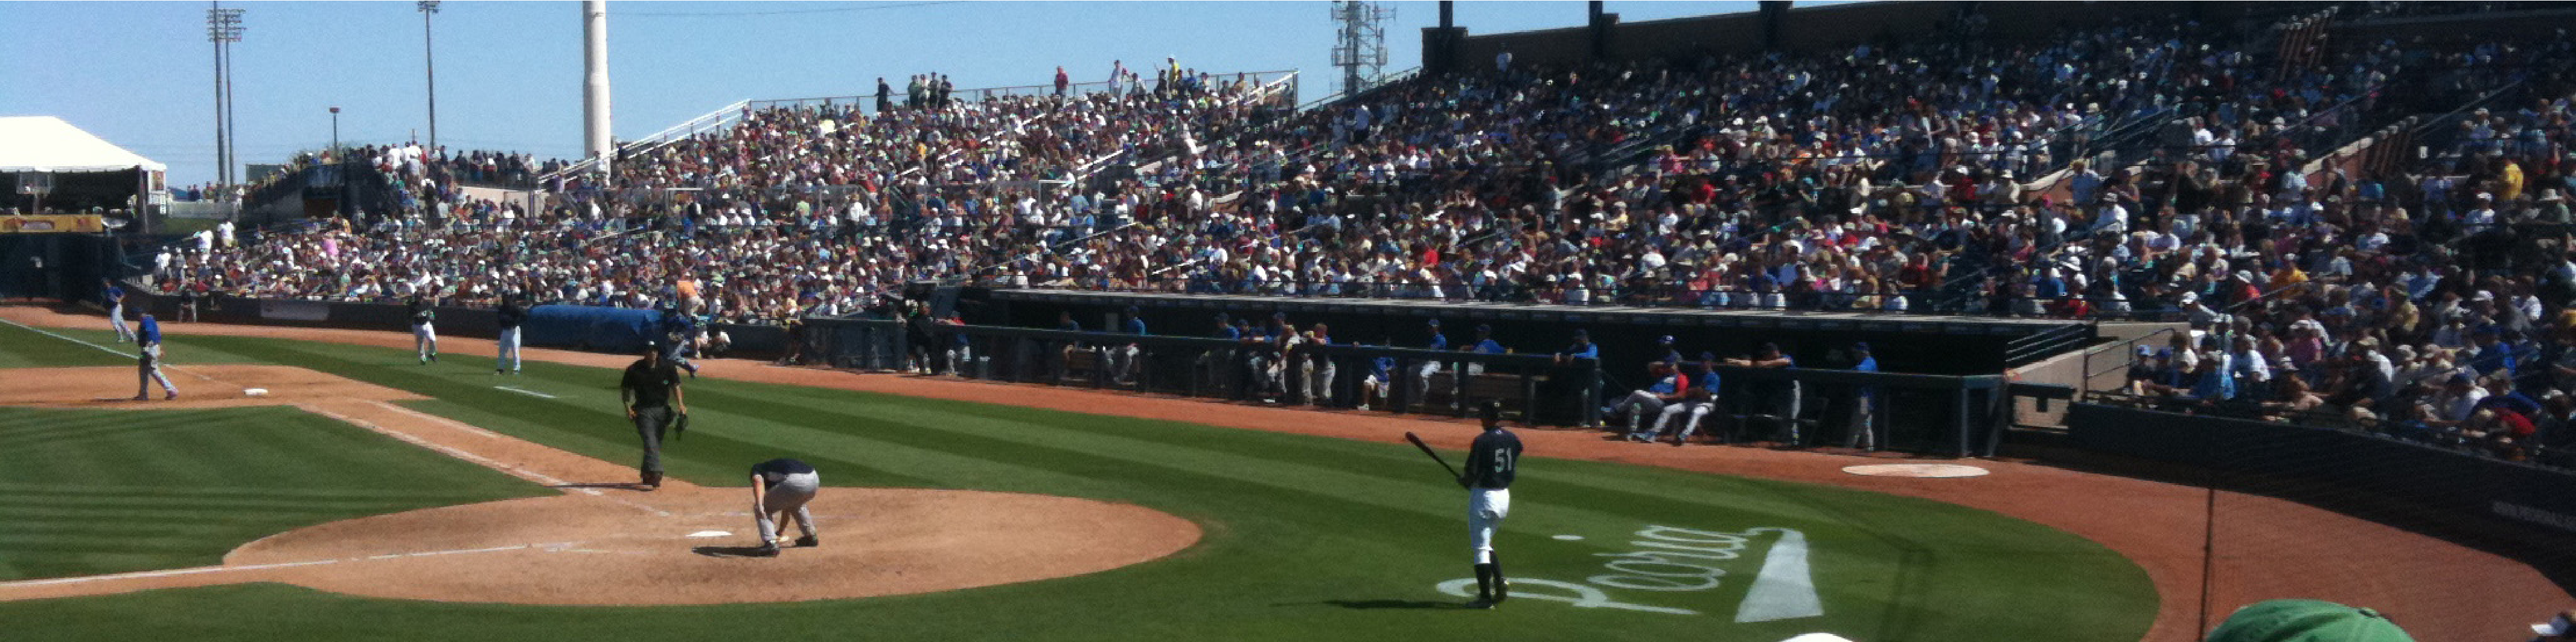
\includegraphics[width=\textwidth]{sampleteaser}
%  \caption{Seattle Mariners at Spring Training, 2010.}
%  \Description{Enjoying the baseball game from the third-base seats. Ichiro Suzuki preparing to bat.}
%  \label{fig:teaser}
%\end{teaserfigure}
\copyrightyear{2019} 
\acmYear{2019} 
%\setcopyright{acmcopyright}
\acmConference[ESEC/FSE '19]{Proceedings of the 27th ACM Joint European Software Engineering Conference and Symposium on the Foundations of Software Engineering}{August 26--30, 2019}{Tallinn, Estonia}
%\acmBooktitle{Proceedings of the 27th ACM Joint European Software Engineering Conference and Symposium on the Foundations of Software Engineering (ESEC/FSE '19), August 26--30, 2019, Tallinn, Estonia}
\acmPrice{15.00}


%
% This command processes the author and affiliation and title information and builds
% the first part of the formatted document.
%\thispagestyle{empty}

\maketitle



\section{Introduction}
Bug localization is a process of locating source code that needs to be changed in order to fix a given bug. 
Manually locating buggy files is not only time-consuming but also prohibitively costly in terms of development efforts \cite{Wang}. This is even more challenging for large software systems. Thus, effective automated approaches are highly warranted for localizing software bugs. 
Traditional Information Retrieval (IR) based bug localization techniques \cite{Saha,Jian} accept a bug report (query) and a subject system as inputs and return a list of buggy entities (e.g., classes, methods). They localize the bugs by simply relying on the \emph{lexical similarity} between a bug report and the source code. 
Hence, they are likely to be affected by the quality and content of a submitted query (i.e., bug report). That is, if the query does not contain adequate information, then the retrieved results might not be relevant at all. As existing findings \cite{parninireval,fse2018masud} suggest, bug reports could be of low quality and could miss the appropriate keywords. 
Thus, lexical similarity alone is likely not sufficient enough for solving the bug localization problem. 

In order to address the limitations of lexical similarity based approaches, several existing studies \cite{Maletic, MarcusMaletic,irmarcus} derive the underlying semantics of a text document by employing Latent Semantic Analysis (LSA). \citeauthor{irmarcus} and colleagues adopt this technology in the context of concept location \cite{irmarcus,MarcusMaletic}, program comprehension \cite{Maletic} and traceability link recovery problems \cite{MarcusLSI}, and reported higher performance than that of the Vector Space Model (VSM) and probabilistic models.
Unfortunately, their approach suffers from a major limitation.
Latent Semantic Indexing (LSI) requires the use of a dimensionality reduction parameter that must be tuned for each document collection \cite{Kontostathis}.
The results returned by LSI can also be difficult to interpret, as
they are expressed using a \emph{numeric spatial representation}.
Other related studies \cite{LukinsBL,Nguyen} adopt Latent Dirichlet Allocation (LDA) for bug localization. However, they are also subject to their \emph{hyper-parameter tuning} and could even be outperformed by much simpler models (e.g., rVSM \cite{Jian}). 
\begin{table*}[t]
	\centering
	\caption{A working example of BLuAMIR}
	\label{tab:workingexample}
	\vspace{-.2cm}
	\resizebox{6.6in}{!}{%
		\begin{threeparttable}
			\begin{tabular}{p{2.5in}|c|c||p{2.5in}|c|c|c|c}
				\hline
				%\begin{tabular}[c]{@{}c@{}}\#Bugs for \\ developing \\ map databases\end{tabular} &
				\multicolumn{3}{c||}{\textbf{VSM (Lexical Similarity Only)}} &
				\multicolumn{5}{c}{\textbf{BLuAMIR (Lexical Similarity + Implicit Association)}}\\
				\hline
				
				\textbf{Retrieved Documents } & 
				\textbf{$\mathbf{S_{LS}}$}  & 
				\textbf{GT}  &
				\textbf{Retrieved Documents } &
				\textbf{$\mathbf{S_{LS}}$}  & 
				\textbf{$\mathbf{S_{Assoc}}$} &
				\textbf{$\mathbf{S_{Total}}$} &
				
				\textbf{GT}\\
				\hline
				\hline
				\texttt{ClasspathLocation.java} & 1.00  & \xmark & \texttt{\textbf{CompletionEngine.java}} & \textbf{0.67}  & \textbf{1.00}  & \textbf{0.80} & \textbf{\checkmark} \\
				\hline
				\texttt{JavaCore.java}  & 0.74 & \xmark & \texttt{AbstractDecoratedTextEditor.java} & 0.69 & 0.73 & 0.71 &  \xmark \\ 
				\hline
				\texttt{SearchableEnvironmentRequestor.java} &  0.73  & \xmark & \texttt{AntEditor.java} & 0.69 & 0.73 & 0.71 &  \xmark\\
				\hline
				\texttt{Compiler.java} &  0.71 & \xmark & \texttt{JavaCore.java} & 0.74 & 0.64 & 0.70 &  \xmark\\
				\hline
				\texttt{AccessRuleSet.java}  & 0.70  & \xmark & \texttt{Engine.java} & 0.70 & 0.70 & 0.70 &  \xmark \\
				\hline
			\end{tabular}
			\centering
			\textbf{GT} = \textbf{G}round \textbf{T}ruth,
			\textbf{$\mathbf{S_{Total}}$} = (1--$\alpha$)$\times$
			\textbf{$\mathbf{S_{LS}}$}
			+$\alpha$$\times$
			\textbf{$\mathbf{S_{Assoc}}$}
			and weighting parameter, $\mathbf{\alpha}$$ = $ 0.4
		\end{threeparttable}
}
\vspace{-.3cm}
\end{table*}

In this paper, we propose a bug localization approach namely \textbf{BLuAMIR} that (1) not only considers \emph{lexical similarity} between a bug report (the query) and the source code (2) but also captures \emph{implicit association} between them from the bug fixing history. First, we determine the lexical similarity between each source document and the query using Vector Space Model (VSM).
Second, we construct association maps between keywords of previously fixed bug reports and their corresponding changed documents using a bipartite graph \cite{bipartite}. Third, we prioritize such source documents that are historically associated with the keywords (from the query at hand) according to these maps. Then, we rank the source code documents based on their \emph{lexical} and \emph{association scores}.
%Thus, our approach caters for the vocabulary mismatch between a bug report (the query) and the source code with implicit association.
Thus, our approach uses implicit association to address the vocabulary mismatch between a bug report (the query) and the source code. 
That is, unlike traditional IR-based bug localization approaches \cite{Jian,Saha}, BLuAMIR can return the buggy documents even if the query does not lexically match with the source code documents. Our approach also does not require the \emph{dimensionality reduction} since we use a finite graph rather than a large sparse term-document matrix \cite{MarcusLSI,MarcusMaletic}.

We evaluate our technique from three different aspects using
three widely used performance metrics and 3,431 bug reports (i.e.,
queries) from four open source subject systems. 
First, we evaluate in terms of bug localization performance metrics, and contrast with two replicated baselines -- Latent Semantic Indexing (LSI) \cite{MarcusLSI} and the basic Vector Space Model (VSM) \cite{vector-space-model}.
BLuAMIR localizes bugs with 9\%--37\% higher accuracy (i.e., Hit@10), 12\%--63\% higher precision (i.e., MAP), and 11\%--64\% higher reciprocal ranks (i.e., MRR) than these baselines (Section  \ref{RQ1answer}).
Second, we compare our technique with three state-of-the-art approaches -- BugScout \cite{Nguyen}, BugLocator \cite{Jian} and BLUiR \cite{Saha} (Section \ref{RQ1answer}).
Our technique can localize bugs with 6\%--54\% higher accuracy (i.e., Hit@5), 4\%--32\% higher precision (i.e., MAP) and 8\%--27\% higher reciprocal ranks (i.e., MRR) than those of the state-of-the-art approaches.
Third, in terms of query-wise improvement, BLuAMIR improves the result ranks of 46.37\% baseline queries from Eclipse subject system and outperforms the baseline VSM approach (Section \ref{RQ1answer}).
Thus, this paper makes the following contributions:
\begin{enumerate}[noitemsep,topsep=0pt]
	\item A novel technique that not only considers the \emph{lexical similarity} between a bug report and the source code but also exploits their \emph{implicit associations} through bug-fixing history for bug localization.
	\item Comprehensive evaluation of the technique using \emph{three} widely used performance metrics and a total of 3,431 bug reports from \emph{four} open source subject systems.
	\item Comparison with not only \emph{two} baselines \cite{vector-space-model,MarcusLSI} but also \emph{three} state-of-the-art approaches -- BugScout \cite{Nguyen}, BugLocator \cite{Jian} and BLUiR \cite{Saha} with statistical tests.
	\item Experimental meta data and our used dataset for  replication and third party reuse.
\end{enumerate}

The rest of the paper is organized as follows-- Section \ref{sec:motivatingexample} discusses a motivating example of our proposed approach, and Section \ref{sec:proposedmethod} presents proposed bug localization method for BLuAMIR, and Section \ref{sec:expANDdiss} focuses on the conducted experiments and experimental results, and Section \ref{sec:threats} identifies the possible threats to validity, and Section \ref{relatedwork}
discusses the existing studies related to our research, and finally,  
Section \ref{sec:conclusionANDfuture} concludes the paper with future plan.



\section{Motivating Example}\label{sec:motivatingexample}
Let us consider a bug report (ID\# 95167) from an Eclipse subsystem namely \texttt{eclipse.jdt.core}. Table \ref{tab:BugInfo} shows the \textit{title} and \textit{description} of the bug report. We capture both fields and construct a baseline query by employing standard natural language preprocessing (e.g., stop word removal, token splitting). Then we execute the query with the Vector Space Model (VSM) and our approach--BLuAMIR, and attempt to locate the buggy source documents.

\small
\begin{table}[!tb]
	\caption{\small An Example Bug Report (\#95167, eclipse.jdt.core)}
	\label{tab:BugInfo}
	\vspace{-.3cm}
	%\centering
	%\begin{center}
	\resizebox{3.25in}{!}{%
		\begin{threeparttable}
		\begin{tabular}{l | p{6.5cm}}
			\hline
			\textbf{Field}  & \textbf{Content} \\
			\hline
			\hline
			Title &  [content assist] Spurious "Access restriction" error during code assist
			\\
			\hline
			Description &  
			(1) OSGi, Runtime, SWT, JFace, UI, Text loaded from head, (2) open type on \texttt{AbstractTextEditor}, (3) at start of createPartContro method, type: PartSite \texttt{<Ctrl+Space>}, and (4) it has no effect in the editor, but the status line flashes in red: Access restriction: The type \texttt{SerializableCompatibility} is not accessible due to restriction on required project \texttt{org.eclipse.swt}. The type name doesn't seem to matter.  ``abcd" has the same effect. 
			I notice that org.eclipse.ui.workbench.texteditor's classpath has an access rule
			forbidding **/internal/** refs.
			\\
			\hline
		\end{tabular}
	\end{threeparttable}
	 
	}
	\vspace{-.4cm}
	%\end{center}
	%\centering
\end{table}
\normalsize



According to the ground truth constructed from bug-fixing history, one source code document (\texttt{CompletionEngine.java}) was changed to fix the reported bug. 
As shown in Table \ref{tab:workingexample}, we see that the \emph{lexical similarity} based approach, VSM, fails to retrieve any buggy source document within the Top-5 positions. On the contrary, our approach, BLuAMIR, complements the \emph{lexical similarity} based ranking with \emph{implicit association} scores, and then returns the target buggy document at the top most position of the result list. This is not only promising but also the best possible outcome that an automated approach can deliver.   

We also investigate why BLuAMIR performs better than VSM in localizing the buggy document(s). Table \ref{tab:workingexample} shows different scores from both approaches. We see that several source documents (e.g., \texttt{ClasspathLocation.java}) that are retrieved by VSM are  
strongly similar to the query. However, such similarity does not necessarily make them buggy. In fact, VSM returns the ground truth document at the lowest position of the Top-10 results (not shown in Table \ref{tab:workingexample}). Thus, \emph{lexical similarity} alone might not be sufficient enough for effective bug localization. However, our approach overcomes such challenge 
by exploiting the \emph{implicit association} between the query and the buggy documents (Section \ref{sec:vsm-assoc-sore}), and returns the target ground truth at the top-most position. Although the lexical similarity is low (e.g., 0.67), our approach correctly identifies the buggy document using its strong implicit association score (e.g., 1.00) with the given query.  

\begin{figure*}
	\centering
	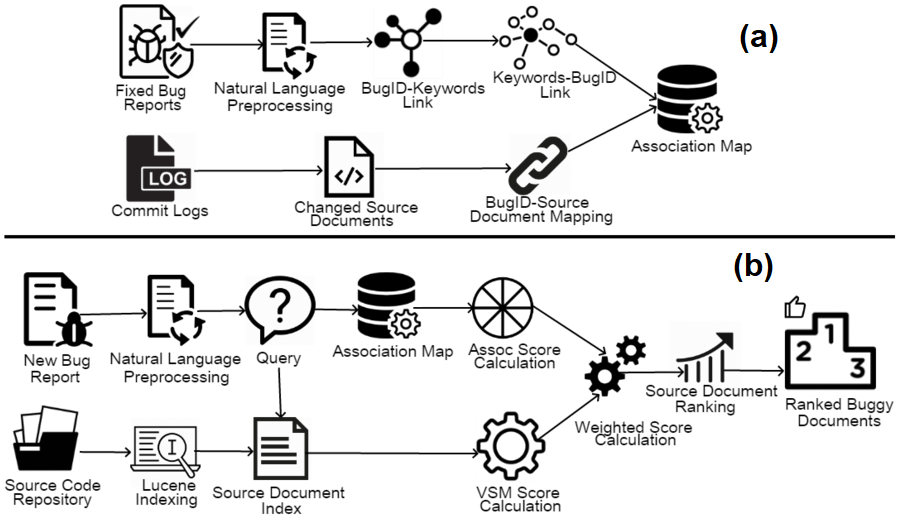
\includegraphics[width=4.8in]{SD6Trans}
	\vspace{-.2cm}
	\caption{Schematic diagram of BLuAMIR--(a) Construction of association map between keywords and source documents,  and (b) Bug Localization using VSM and implicit association}
	\label{fig:systemDiagram}
	\vspace{-.2cm}
\end{figure*}

\section{BLuAMIR: Proposed Approach for Bug Localization} \label{sec:proposedmethod} 
Figure \ref{fig:systemDiagram} shows the schematic diagram of our proposed approach.
Furthermore, Algorithms \ref{algo:map}, \ref{algo:localization} show the pseudo-code of our approach. 
%Our proposed approach combine lexical similarity and co-occurence similarity measure.  \citet{Jian} proposed BugLocator based on two different similarity scores- one is rVSM score and the other one is Simi score. 
First, we (a) construct an association map between the bug reports and their corresponding changed source documents with the help of bug-fixing history.
%where the inherent association between past bug reports and their changed documents are leveraged.
%In BLuAMIR, we follow two different approach for computing source code ranks.
Then we (b) retrieve buggy source code documents for a given query (bug report) by leveraging not only their lexical similarity but also their implicit associations derived from the association map above.   
%based on two different scores - VSM and association.  
%However, we have divided our approach into two different sections or parts- 1) calculate rVSM and Simi scores or VSM score and co-occurence measure and 2) combine all three or two scores in order to localize recommended buggy source files for a given newly reported bug. 
%As we have combined two existing scores with our proposed word co-occirence score, 
We discuss different parts of our proposed approach in the following sections.

\subsection{Construction of Keyword--Document Association Map}\label{sec:MapConstruction}
We construct an association map between keywords from previously fixed bug reports and their corresponding changed source documents.
The map construction involves three steps.
We not only show different steps of our map construction  (Fig. \ref{fig:systemDiagram}-(a)) but also provide the corresponding pseudo-code (Algorithm \ref{algo:map}). We discuss each of these steps as follows:

%refer to both figure and algorithm in the texts. 


\textbf{(1) Extraction of Keywords from Bug Reports:} We collect \emph{title} and \emph{description} of each bug report from a subject system.  
Then we perform standard natural language preprocessing, and remove punctuation marks, stop words and small words (i.e., \emph{length $\le$ 2}) from them. Stop words convey very little semantics in a sentence. 
%Stemming extracts the root of each of the word. 
We use appropriate regular expressions to discard all the punctuation marks and 
a standard list\footnote{{1}https://www.ranks.nl/stopwords} for stop word removal. 
%and Porter Stemming stemmer\footnote{{2}http://tartarus.org/martin/PorterStemmer/} for stemming. 
Finally, we select a list of remaining keywords from each bug report. 
We then create a \emph{map} (e.g., $M_{bk}$) between the ID of each bug report and their corresponding keywords (Lines 5--6, Algorithm \ref{algo:map}).   
We also construct an \emph{inverted index} (e.g., $M_{kb}$) between keywords and their corresponding bug report IDs (Lines 7-8, Algorithm \ref{algo:map}) by using the above constructed map.

\textfloatsep5pt
\begin{algorithm}[!tb]
	\caption{Construction of Association Map}
	\label{algo:map}
	\begin{algorithmic}[1]
		\Procedure{MapConstruction}{$BRC$, $BFC$}
		
		\LineComment{$BRC$: a collection of past bug reports}
		
		\LineComment{$BFC$: bug-fix commit history}
		\State $M_{KS} \gets$ \{\}
		\Comment{an empty association map}
		%\Comment{creating adjacency map database from the bug reports collection}
		%\State $MAP_{adj} \gets$ createAdjacencyDatabase($BRC$)
		%\Comment{creating a map that links keywords into their bug ids}
		\LineComment{Create map between Bug ID and keywords}
		\State $M_{bk} \gets$ createBugIDtoKeywordMap($BRC$)
		
		\LineComment{Create an inverted index between keywords and ID}
		\State $M_{kb} \gets$ createKeywordtoBugIDMap($M_{bk}$)
		
		
		\LineComment{Map between Bug ID and changed source documents}
		\State $M_{bs} \gets$ createBugIDtoSourceMap($BFC$)
		
		\LineComment{Mapping keywords to the changed source documents}
		%\LineComment{preprocess the collected keywords}
		%\For{Keyword $K_i \in$ $K$}
		\State $KW \gets$ collectKeywords($M_{kb}$)
		
		
		\For{Keyword $kw$ $\in$ $KW$}
		\State $ID_{kw} \gets$ extractBugIDs ($kw$, $M_{kb}$)
		\For{BugID $id_{kw}$ $\in ID_{kw}$}
		\LineComment{Get the linked source documents}
		\State $SD_{link} \gets$ getDocuments($M_{bs}$, $id_{kw}$)
		%\Comment{Retrieve associated source from $MAP_{bs}}$
		%\State $MAO_{BUG_{id}} \gets$ linkSourceCodeFiles$Adj_{T_i}, Adj_{K_j}$) 
		\LineComment{Map all source documents to this keyword}
		\State $M[kw].link \gets \{M[kw].link~~\cup~~SD_{link}$\}
		\EndFor
		\EndFor
		
		\LineComment{collect all keyword--source document mappings}
		\State $M_{KS} \gets$ $M[KW]$ 
		
		
		%\LineComment{put them into map}
		%\State $MAP \gets$ mapping()
		\State \textbf{return} $M_{KS}$
		\EndProcedure
	\end{algorithmic}
\end{algorithm}
%\vspace{-1cm}


\textbf{(2) Extraction of Changed Source Documents from Bug-Fix Commits:}
We analyse the version control history of each subject system, and identify the bug-fixing commits using appropriate regular expressions \cite{bugid,Wang2}.
In particular, we go through all the commits and identify such commits that contain keywords related to bug fix or resolution in their title messages.
Then, we collect the \emph{changeset} (i.e., list of changed documents)
from each of these bug-fix commits, and construct a Bug ID--document map (e.g., $M_{bs}$) for our study (Lines 9--10, Algorithm \ref{algo:map}). 
%Thus, for experiments, we collect not only the actual change requests from the reputed subject systems but also their solutions which were applied in practice by the developers \cite{SHaiduc}. 
We use several
utility commands such as \texttt{git, clone} and \texttt{log} on Git-based repository of each system for collecting the above information.

%\setlength{\textfloatsep}{12.0pt plus 2.0pt minus 4.0pt}

%This step is done line 7 of Algorithm \ref{algo:map}. 
%Each of these commit messages presents other information such as the ID of bug report for which it was created and the links of the corresponding changed source code files. 
%We then construct a linking relationship between each fixed bug report ID into their changed source code files, which is mentioned in line 4 of Algorithm \ref{algo:map}.

\textbf{(3) Construction of Mapping between Keywords and Changed Source Documents:}
The above two steps deliver (1) an inverted index ($M_{kb}$) that maps each individual keyword to numerous bug report IDs, and (2) a map ($M_{bs}$) that links each bug report ID to its corresponding changed source documents based on the bug-fixing history.
%It should be noted each bug-fixing commit establishes an inherent relationship between its changed documents and the target bug report. 
Since both of these maps are connected through bug report IDs,
keywords from each bug report also enjoy an implicit, transitive relationship with the corresponding changed source code documents.
We leverage such transitive relationship and construct a bipartite graph (e.g., Fig. \ref{fig:BipartiteGraph}) by explicitly connecting the keywords from each bug report to their corresponding changed source documents (Lines 11--22, Algorithm \ref{algo:map}).
%We construct the bipartite graph (i.e., discussed bellows) between keywords collected from a bug report and buggy source document links.
Here, one or more keywords could be linked to single buggy source code document. Conversely, single source document could also be linked to one or more keywords from multiple bug reports. 

\textbf{An Example Association Map with Bipartite Graph:} In Mathematics, \emph{bipartite graph} is defined as a special graph that   
(1) has two disjoint sets of nodes and a set of edges and (2) each of its edges connects two nodes from the two different sets but not from the same set \cite{bipartite}.  
%only edges are between those two groups, and there are no edges between vertices within the same group. 
\begin{table}[!tb]
	\caption{Example Bug Report (\#322401, eclipse.ui.platform)}
	\label{tab:BugInfo2}
	%\centering
	%\begin{center}
	\vspace{-.3cm}
	\resizebox{3.3in}{!}{%
		\begin{tabular}{ p{2cm} | p{6.0cm}}
			\hline
			\textbf{Field}  & \textbf{Content} \\
			\hline
			\hline Title &
			[LinkedResources] Linked Resources properties page should have a Remove button
			\\ \hline
			Description &  
			Project properties $>$ Resource $>$ Linked Resources:
			Especially for invalid locations, a Remove button would be handy to remove one or multiple links. \\
			\hline
		\end{tabular}
	}
	\vspace{-.2cm}
	%\end{center}
	%\centering
\end{table}
\begin{figure}
	\centering
	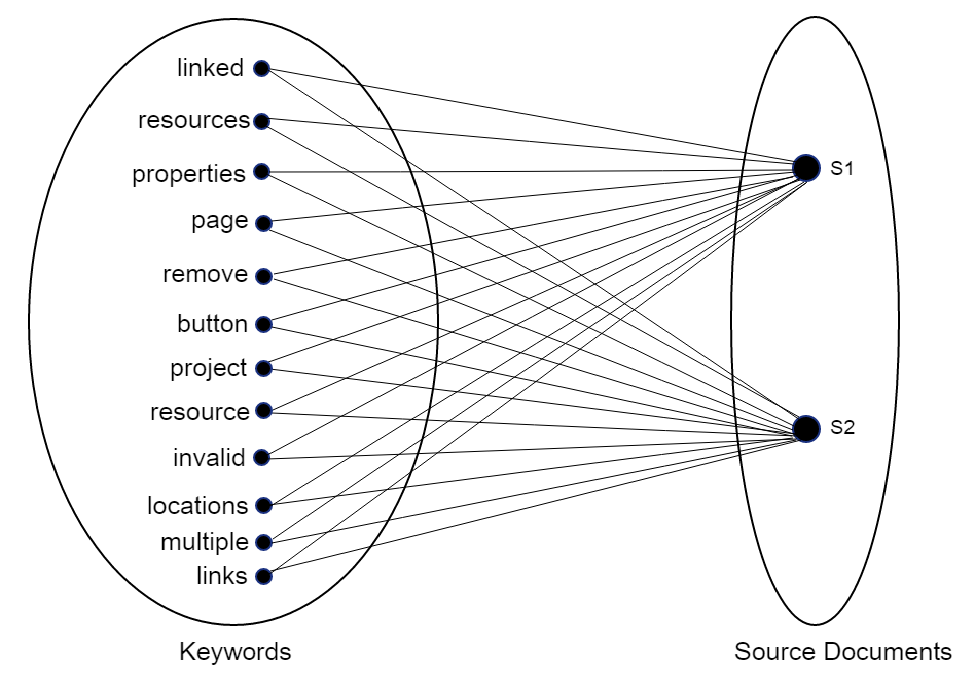
\includegraphics[width=3.3in]{BGraph5}
	\caption{An example association map using bipartite graph}
	\label{fig:BipartiteGraph}
	\vspace{.2cm}
\end{figure}
In our study, these two sets correspond to keywords (from bug reports) and source code documents. 
Thus, no connection between any two keywords or any two source documents is allowed.
%Hence, nether two keywords nor two source files can be connected. There exist only one type of valid link, which can be established between a keyword and its corresponding sources. 
We construct an example bipartite graph for a bug report (ID 322401) from Eclipse UI Platform. Table \ref{tab:BugInfo2} shows the \textit{title} and \textit{description} of the bug report. According to the bug-fix history, these two documents - \texttt{\textbf{S$_1$}:IDEWorkbenchMessages.java} and \texttt{\textbf{S$_2$}: LinkedResourceEditor.java}-- constitute the ground truth of the bug report above. Fig. \ref{fig:BipartiteGraph} shows the bipartite graph for the bug report along with its ground truth. We see that twelve keywords and two source documents represent the two sets of nodes and each node is connected to all the nodes from another set. In our approach, we iteratively update such a bipartite graph with new nodes and new connections generated from each of the bug reports of a subject system (Lines 15--20, Algorithm \ref{algo:map}). 

\subsection{Bug Localization using VSM and Implicit Association}\label{sec:vsm-assoc-sore}
Fig. \ref{fig:systemDiagram}-(b) shows the schematic diagram
and Algorithm \ref{algo:localization} presents the pseudo-code
of our bug localization component.
We have constructed an association map (e.g., $M_{KS}$) that connects the keywords from a bug report to its corresponding changed source documents (Section \ref{sec:MapConstruction}). We leverage this association map, and return a list of buggy source documents that are not only lexically similar but also strongly associated with a given query (i.e., bug report at hand). We thus calculate two different scores for each candidate source document and then suggest the Top-K buggy documents as follows:

%\textfloatsepem
\begin{algorithm}[!tb]
	\caption{Proposed Bug Localization Approach}
	\label{algo:localization}
	\begin{algorithmic}[1]
		\Procedure{BugLocalization}{$Q$, $SCrepo$, $M_{KS}$}
		
		\LineComment{$q$: a given query (bug report)}
		\LineComment{$SCrepo$: a source code repository}
		\LineComment{$M_{KS}$: keyword-source document  map}
		
		
		\State $RL \gets$ \{\}
		\Comment{list of buggy source documents}
		
		\LineComment{Create an index of source documents}
		\State $Index \gets$ createLuceneIndex($SCrepo$)
		\LineComment{Collect lexically similar documents}
		\State $VSM\gets$ getLexSimDocuments($q$, $Index$)
		\LineComment{Collecting associated documents}
		\State $Assoc\gets$ getAssociatedDocuments($q$, $M_{KS}$)
		
		%\Comment{Linking keywords into change source code}
		%\LineComment{preprocess the collected keywords}
		%\For{Keyword $K_i \in$ $K$}
		%\State $SC_{Assoc} \gets$ %collectSCodeWithAssocScore($Score_{Assoc}$)
		\LineComment{Combine both candidate document lists}
		\State $C\gets$\{$VSM.docs$ $\cup$ $Assoc.docs$\} 
		
		\For{SourceDocument $d\in C$}
		\LineComment{Combine lexical and association scores}
		\State $C[d].score\gets VSM[d].score$
		\State $C[d].score\gets$ $C[d].score$+$Assoc[d].score$
		\EndFor
		\LineComment{Sort the candidates and collect Top-K documents}
		\State $RL\gets$ getTopKDocuments(sortByScore($C$))
		\State \textbf{return} $RL$
		\EndProcedure
	\end{algorithmic}
\end{algorithm}

\textbf{Lexical Similarity Score:}
Source code documents often share a major \emph{overlap} in the vocabulary with a submitted bug report. Many of the existing studies \cite{Jian,Saha,Saha2,Wang2} consider such vocabulary overlap (i.e., lexical similarity) as a mean to localize the buggy source documents. These studies generally employ Vector Space Model (VSM) \cite{vector-space-model} for calculating the vocabulary overlap. VSM is a classical approach for constructing vector representation of any text document (e.g., bug report, source code document) \cite{vector-space-model}. First, it encodes a document collection (a.k.a., corpus) using a term-by-document matrix where each row represents a term and each column represents a document. Second, each matrix cell is defined as the frequency of a term within a specific document (i.e., term frequency). 
Thus, \emph{lexical similarity} between a given query (bug report) and a candidate source document is computed as the \emph{cosine} or \emph{inner product} between their corresponding vectors from the matrix.
Since term frequency (TF)-based vector representation might be biased toward large documents, several studies \cite{Jian,Saha} also represent their vectors using TF-IDF. It stands for term frequency times inverse document frequency.
TF-IDF assigns higher weights to such terms that are frequent within a document but not frequent across the whole document collection \cite{Salton}.       
%The weight of a term in a document increases with its occurrence frequency in this specific document and decreases with its occurrence frequency in other documents.
%In our proposed approach we have used both classical Vector Space Model (VSM)  and revised Vector Space Model (rVSM) proposed by \citet{Jian} in order to index and rank source code files. 

%\setlength{\textfloatsep}{12.0pt plus 2.0pt minus 4.0pt}

In classic VSM, term frequency $tf(t,d)$ and inverse document frequency $idf (t)$ are defined as follows:
\begin{equation*}
tf(t,d)=\frac{f_{td}}{\#terms},~~idf(t)=1+log(\frac{\#docs}{n_{t}})
\end{equation*}
Here $f_{td}$ refers to the frequency of each unique term {$t$} in a document {$d$}, $n_t$ denotes the document frequency of term $t$, $\#docs$ is the total number of documents in the corpus and $\#terms$ refers to the total number of unique terms in the corpus.  
%and {$f\textsubscript{td}$} is the number of times term {$t$} appears in document {$d$}.
Thus, the lexical similarity between a given query $q$ (i.e., given bug report) and a candidate source code document $d$ is calculated as follows:
\begin{multline*}\label{VSMequation}
lexicalSimScore(q,d)= cosine(q,d) =
\\
\frac{\sum_{t\epsilon \{q\bigcap d\}}tf(t,q)\times tf(t,d)\times idf(t)^{2}
}{\sqrt{\sum_{t\epsilon q}(tf(t,q)\times idf(t))^2}\times
	\sqrt{\sum_{t\epsilon d}(tf(t,d)\times idf(t))^2}}
\end{multline*}
%Here, {$\#terms$} refers to the total number of terms in a document collection. 
Here $lexicalSimScore$ takes a value between 0 and 1 where 0 means total lexical dissimilarity and 1 means strong lexical similarity between the query $q$ and the candidate source code document $d$. We use \emph{Apache Lucene} for first creating the corpus index and then for calculating the above lexical similarity (Lines 6--9, Algorithm \ref{algo:localization}).

\textbf{Implicit Association Score:} We analyse implicit associations between a given query (bug report) and each candidate source document using our constructed association map (from Section \ref{sec:MapConstruction}). In this map, while each keyword could be linked to multiple candidate documents, each document could also be linked to multiple keywords across multiple bug reports. 
We perform standard natural language preprocessing on a given query, and extract a list of query keywords.
We then identify such source documents in the map that are linked to each of these keywords. Since these links were established based on the bug-fixing history, they represent an \emph{implicit relevance} between the keywords and the candidate source documents. It should be noted that such relevance does not \emph{warrant for any lexical similarity}.
%We assume these files are relevant because we created the map between the content of bug reports and their buggy source files for previously fixed bug reports. 
We analyse such links for all the keywords ($\forall t\in q$) of a search query $q$, and determine how frequently each candidate source document $d$ was associated with these keywords in the past as follows: 
\begin{equation*}\label{CoOccequation}
associationScore(q,d)=\sum_{t\in q}\sum_{id\in ID_t} \#link(t,d,id)
\end{equation*}
Here $\#link(t,d,id)$ returns the frequency of association between the keyword $t\in q$ and the source document $d$ for the bug report with ID $id\in ID_t$.   
%across the bug-fixing history of a subject system. 
That is, $associationScore$ assigns a score to each candidate document by capturing their historical co-occurrences with the query keywords across the bug-fixing history of a system.

\textbf{Final Score Calculation:} The above two sections deliver two different scores (\emph{lexical similarity}, \emph{implicit association}) for each of the candidate source code documents. Since these scores could be of different ranges, we normalize both of them between 0 and 1. We then
combine both scores using a weighted summation, and calculate the final relevance score for each candidate document $d$ (Lines 14--18, Algorithm \ref{algo:localization}) as follows:
\begin{multline*}\label{equationVSMme}
FinalScore(q,d)=(1-\alpha )\times Norm(lexicalSimScore)+ \\
\alpha \times Norm(associationScore)
\end{multline*}
Here, the weighting factor $\alpha$ varies from 0.2 to 0.4, and
the detailed justification is provided in the discussion section (Section \ref{RQ1answer}). 

Once the final score is calculated for each of the candidate source documents from the corpus, we return the only Top-K (1$\le$K$\le$10) results as the buggy source documents for the given query $q$ (i.e.,  Lines 19--21, Algorithm \ref{algo:localization}).

\section{Experiment} \label{sec:expANDdiss}
We evaluate our technique in three different aspects using
three widely used performance metrics and 3,431 bug reports (i.e.,
queries) from four open source subject systems. We compare not only with two baseline techniques \cite{vector-space-model,MarcusLSI} but also three state-of-the-art studies \cite{Nguyen,Jian,Saha} from the literature. In particular, we answer three research questions with our experiment as follows: 
\begin{itemize}
	\item \textbf{RQ$_1$}: How does the proposed approach perform in bug localization compared to the baseline approaches? 
	\item \textbf{RQ$_2$}: Can the proposed approach outperform the state-of-the-art studies in bug localization?
	\item \textbf{RQ$_3$}: (a) Can implicit association make any significant difference in IR-based bug localization? and (b) can BLuAMIR overcome the challenges with large documents?   
\end{itemize}

\begin{table}[!tb]
	\caption{Experimental Dataset}
	\label{tab:DDSl}
	%\centering
	\vspace{-.3cm}
	%\begin{center}
	\resizebox{3.35in}{!}{%
		\begin{tabular}{ l| c | p{2.7cm} | c | c }
			\hline
			\textbf{Project} & \textbf{Version} & \textbf{Study Period}& \textbf{\#Bugs} & \textbf{\#Documents}\\
			\hline
			%{Eclipse Platform Ant} & Popular IDE for Java & Nov 2001 - April 2010 & {3855} & 11732\\ \hline
			\hline
			
			Eclipse & v3.1  & Oct 2004 - Mar 2011 & {3071} & 11,831\\ \hline
			SWT &  v3.1 & Oct 2004 - Apr 2010 & 98 &  484\\ \hline
			AspectJ & - & July 2002 - Oct 2006 & 244 & 3519 \\ \hline
			ZXing & - & Mar 2010 - Sep 2010 & 20 & 391 \\
			\hline
		\end{tabular}
	}
	%\vspace{-.3cm}
	%\end{center}
	%\centering
\end{table}


\subsection{Experimental Dataset}\label{sec:dataset}
Table \ref{tab:DDSl} shows our experimental dataset. We use a total of 3,431 bug reports from four open source systems--Eclipse, AspectJ, SWT and ZXing--for our experiment. These systems are collected from two existing, frequently used public benchmarks \cite{Jian,Saha}. 
%In order to evaluate our proposed tool we have used the same four dataset that \citet{Jian} and \citet{Saha} used
%to evaluate BugLocator and BLUiR respectively. This dataset contains 3479 bug reports in total from four popular open source projects–Eclipse, SWT, AspectJ and ZXing along with the information of fixed files for those bugs.
%The detail of our dataset is presented in \ref{tab:DDSl}. 
\emph{Eclipse} is a well-known large-scale system which is frequently used in empirical Software Engineering research.
\emph{SWT} is a component of Eclipse IDE.
\emph{AspectJ} is a part of iBUGs dataset provided by University of Saarland. 
ZXing is an android based system maintained by Google. We collect \emph{title} and \emph{description} from each of these 3,431 bug reports. We perform standard natural language preprocessing on them, and remove stop words, punctuation marks, and small words from them. Then each of these preprocessed bug reports is used as the \emph{baseline query} for our experiment. 

%as generally done 
%preprocess them with standard n use them as queries for the bug localization.

%We create quires from each bugs considering their title and short summary (i.e., description).

\textbf{Ground Truth Selection:} We analyse the bug-fixing commits from each subject system, and select the ground truth for our experiment. In particular, we go through all commit messages of a system and identify such commits that deals with bug fixing or resolution (i.e., bug fixing commits) using appropriate regular expressions \cite{bugid}. We then extract the changed source documents from each of these commits, and map them to the fixed bug ID. Such changed documents are then used as the \emph{ground truth} for the corresponding bug reports (i.e., queries). The same approach has been widely used by the literature \cite{Saha2,Wang2,Jian} for the ground truth selection. 

%track Bug IDs associated with examined source code files. Then we construct the association map between keywords extracted from bug reports and their source code links. During creating the map we have noticed some bug reports do not contain their fixed source files in codebase. So, we discarded those bug reports which yield total 3431 bug reports as depicted in table \ref{tab:DDSl}.



\subsection{Performance Metrics}\label{sec:pmetrics}
%To measure the effectiveness of the proposed bug localization approach, we use the following metrics:
We choose three performance metrics for evaluation and validation. These metrics have been widely used by the relevant literature \cite{Jian, Saha}. Thus, they are highly appropriate for our experiments as well. They are defined as follows:

\textbf{Recall at Top K / Hit@K:} It represents the percentage of bug reports for each of which at least one ground truth buggy document is successfully retrieved within the Top-K results. 
%We analyse only Top-10 results for each query, and thus, $K$ could be 1, 5 or 10.  
The higher the Hit@K value is, the better the bug localization performance is.

\textbf{Mean Reciprocal Rank (MRR):}
The reciprocal rank of a query is the multiplicative inverse of the rank of the first buggy document within the result list. Hence, mean reciprocal rank is calculated as the mean of reciprocal ranks of a set of queries $Q$ as follows:
\begin{equation*}
MRR(Q) = \frac{1}{\left | Q \right |}\sum_{q\in Q}\frac{1}{firstRank(q)}
\end{equation*}
where $firstRank(q)$ is the rank of the first buggy source document within the returned result list for a query $q\in Q$. Reciprocal rank takes a value between 0 and 1. Here, 0 value suggests that no buggy document is retrieved whereas 1 value suggests that the first buggy document is retrieved at the top most position of the result list.

\textbf{Mean Average Precision (MAP):}
Mean Average Precision is a commonly used metric for evaluating the ranking approaches. Unlike MRR, it considers the ranks of all buggy documents retrieved in the result list into the consideration. 
%Hence, MAP emphasizes all of the buggy files instead of only the first one.
%MAP for a set of queries is the mean of the average precision scores for each query. 
Average Precision of a query $q$ can be computed as follows:
\begin{equation*}
AP(q)=\sum_{k=1}^{K}\frac{P(k)\times buggy(k)}{|R|},~~P(k)=\frac{\#buggyDocs}{k}
\end{equation*}
where $k$ is a rank in the ranked results, $K$ is the number of retrieved documents, and $R$ is the set of true positive instances. $buggy(k)$ function indicates whether the $k_{th}$ document is buggy or not. $P(k)$ returns the calculated precision at a given rank position. Since AP is a metric for single query $q$, MAP can be calculated for a set of queries $Q$ as follows:
\begin{equation*}
MAP(Q) = \frac{1}{|Q|}\sum_{q\in Q}AP(q)
\end{equation*}
MAP takes a value between 0 and 1. The higher the metric value is, the better the bug localization performance is.

\subsection{Evaluation \& Validation}\label{RQ1answer}
We use a total of 3,431 bug reports from four subject systems (Section \ref{sec:dataset}) and evaluate our approach using three performance metrics (Section \ref{sec:pmetrics}). We employ 10-fold cross validation, and the whole bug report collection is divided into 10 folds. Out of these 10 folds, 
nine folds are used for training (i.e., construct of association map) and the remaining fold is used for testing (i.e., bug localization). We repeat this process 10 times, determine our performance each time, and then report the average performance of our approach. In the following sections, we discuss our experimental results and answer our research questions (RQ$_1$, RQ$_2$) as follows:

\textbf{Answering RQ$\mathbf{_1}$--Comparison with Baseline Approaches:}
We compare the performance of BLuAMIR with two baseline approaches -- Vector Space Model (VSM) \cite{vector-space-model} and Latent Semantic Indexing (LSI) \cite{MarcusLSI}. We replicate both approaches in our development environment, evaluate with our dataset, and then determine their performance. We discuss the comparison with these baselines in details as follows: 

\begin{figure}
	\centering
	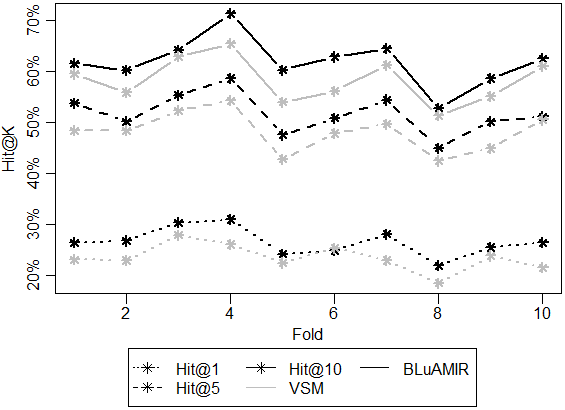
\includegraphics[width=3in]{hitk-vsm-proposed}
	\vspace{-.3cm}
	\caption {Comparison between baseline VSM and proposed approach, BLuAMIR, in Hit@K}
	\label{fig:VSM+AssoTopK}
	\vspace{-.3cm}
\end{figure}

\begin{figure}
	\centering
	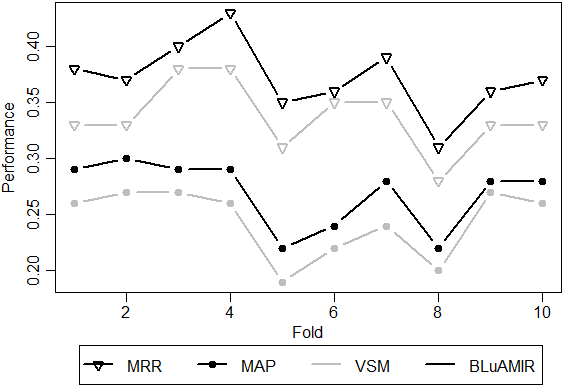
\includegraphics[width=3in]{mrr-map-vsm-proposed}
	\vspace{-.3cm}
	\caption {Comparison between baseline VSM and proposed approach, BLuAMIR, in MRR and MAP}
	\label{fig:VSM+AssoTop-MRR-MAP}
	\vspace{-.1cm}
\end{figure}


\begin{table}[!tb]
	\centering
	\caption{Comparison between Baseline VSM and BLuAMIR}
	\vspace{-.3cm}
	\label{tab:Performance2}
	\resizebox{3.35in}{!}{%
		\begin{tabular}{c|c|c|c|c|c|c}
			\hline
			%\begin{tabular}[c]{@{}c@{}}\#Bugs for \\ developing \\ map databases\end{tabular} &
			
			\begin{tabular}[c]{@{}c@{}} \textbf{\#Bugs} \\ \end{tabular} & 
			\begin{tabular}[c]{@{}c@{}}\textbf{Approach} \\  \end{tabular} 
			& 
			\begin{tabular}[c]{@{}c@{}}\textbf{Hit@1}\end{tabular} & \begin{tabular}[c]{@{}c@{}}\textbf{Hit@5}\end{tabular} & \begin{tabular}[c]{@{}c@{}}\textbf{Hit@10}\end{tabular} & 
			\textbf{MRR} 
			& \textbf{MAP} \\ \hline \hline
			%			\multirow{2}{*}{1}& VSM & 23.67& 46.59&56.97& 0.33 & 0.32 \\ \cline{2-7}
			%			& VSM + Association & 28.40                                               & 51.77                                            & 60.06                                                &   0.38  & 0.36 \\ \hline
			%			\multirow{2}{*}{2}                                                                               & VSM & 24.62 & 48.05 & 57.96 & 0.34 & 0.34 \\  \cline{2-7}  &VSM + Association                                                                    & 27.63                                               & 53.15                                              & 61.26                                             &   0.38  &   0.37  \\ \hline
			%			\multirow{2}{*}{3}                                                                               & VSM & 20.78 & 40.96 & 51.20 & 0.30 & 0.29 \\  \cline{2-7}   &VSM + Association                                                                      & 23.12                                            & 46.85                                            & 59.76                                             &   0.34  &  0.32   \\ \hline
			%			\multirow{2}{*}{4}                                                                               & VSM & 22.52 & 42.94 & 53.75 & 0.32 & 0.31 \\   \cline{2-7} &VSM + Association                                                                    & 23.42                       & 49.25                       & 61.56                                                &  0.35   &  0.33  \\  \hline
			%			\multirow{2}{*}{5}                                                                               & VSM & 27.33 & 52.25 & 63.36 & 0.38 & 0.35 \\   \cline{2-7} &VSM + Association                                                                   & 29.73                                                 & 53.15                                                 & 62.16                                                  &  0.39   & 0.36     \\  \hline
			%			\multirow{2}{*}{6}                                                                               & VSM & 25.00 & 50.60 & 60.84 & 0.36 & 0.34 \\  \cline{2-7}  &VSM + Association
			%			&26.13 &
			%			51.65 &
			%			62.76 & 0.37 &
			%			0.35     \\  \hline 
			%			\multirow{2}{*}{7}                                                                               & VSM & 29.82 & 54.52 & 66.27 & 0.40 & 0.38 \\  \cline{2-7}  &VSM + Association
			%			
			%			&35.43 &
			%			60.96 &
			%			72.07 & 0.46 &
			%			0.44     \\  \hline
			%			\multirow{2}{*}{8}                                                                               & VSM & 27.79 & 51.36 & 60.73 & 0.38 & 0.36 \\  \cline{2-7}  &VSM + Association
			%			&36.64 &
			%			58.86 &
			%			67.87 & 0.46 &
			%			0.43    \\  \hline
			%			\multirow{2}{*}{9}                                                                               & VSM & 29.13 & 52.55 & 64.86 & 0.39 & 0.36 \\  \cline{2-7}   &VSM + Association
			%			&29.13 &
			%			61.86 &
			%			69.97 & 0.42 &
			%			0.40    \\  \hline
			%			\multirow{2}{*}{10}                                                                               & VSM & 19.03 & 39.58 & 51.34 & 0.28 & 0.26 \\  \cline{2-7}  &VSM + Association
			%			&24.62 &
			%			51.05 &
			%			63.06 & 0.36 &
			%			0.34    \\ \hline \hline
			\multirow{2}{*}{3071}                                                                               & VSM & 23.09\% & 47.54\% & 57.57\% & 0.33 & 0.24 \\  \cline{2-7}   & BLuAMIR     & 27.45\%                                                 & \textbf{53.79}\%                                                 & \textbf{63.30}\%                                                  &   \textbf{0.38}  &  0.27    \\ 
			\hline
		\end{tabular}
		
	}
	%\vspace{-.3cm}
	\centering
\end{table}

\textbf{Baseline VSM vs BLuAMIR:} While VSM approach simply relies on the lexical similarity between a given query (bug report) and the source code document, our approach additionally considers their implicit associations based on the bug-fixing history.
We thus compare BLuAMIR with VSM, and investigate whether the addition of association score could improve the overall bug localization performance or not. Table \ref{tab:Performance2} and Figures \ref{fig:VSM+AssoTopK}, \ref{fig:VSM+AssoTop-MRR-MAP} show the comparison between VSM and our approach for \emph{Eclipse} system. From Table \ref{tab:Performance2}, we see that the baseline VSM achieves only 23\% Hit@1, 48\% Hit@5 and 58\% Hit@10. On the contrary, our approach achieves 28\% Hit@1, 54\% Hit@5 and 63\% Hit@10 which are 19\%, 13\% and 10\% higher respectively. BLuAMIR also achieves 15\% higher MRR and 13\% higher MAP than the baseline measures. Since our experiment involves 10-fold cross validation, we also compare our performance with that of baseline VSM for each of these folds. As shown in Fig. \ref{fig:VSM+AssoTopK}, we see that our Hit@K is better than the baseline for each fold of dataset. Fig. \ref{fig:VSM+AssoTop-MRR-MAP} shows how BLuAMIR outperforms the baseline VSM in MRR and MAP respectively for each of these folds. We also perform Wilcoxon Signed-Rank tests, and found that BLuAMIR achieves statistically significant improvement over the baseline in terms of both MRR (i.e., \emph{p-value}=0.005$<$0.05) and MAP (i.e., \emph{p-value}=0.005$<$0.05).

\textbf{Baseline LSI vs BLuAMIR:} Traditional VSM often suffers from vocabulary mismatch problem. Latent Semantic Indexing (LSI)
attempts to overcome such problem by extracting the underlying meaning of a document rather than simply relying on the individual words from the document. As existing study \cite{LSIindexing} suggests, individual words often do not provide reliable evidence about the conceptual topic or meaning of a document. LSI has been used for document retrieval in several Software Engineering contexts \cite{MarcusLSI,MarcusMaletic} which makes it an attractive baseline for our evaluation. We replicate LSI in our development environment following these steps. First,    
we create a term-by-document matrix by capturing both bug reports (queries) and source code documents from a subject system. Second, 
we apply Singular Value Decomposition (SVD) on this matrix, and construct a subspace (i.e., LSI subspace) \cite{SaltonMIR}. 
Third, we compute cosine similarity between queries (bug reports) and candidate source documents using corresponding vectors from  this subspace. Fourth, Top-K source code documents are then returned for each given query (bug report) based on their similarity.  
We compare BLuAMIR with baseline LSI using three subject systems-- \emph{AspectJ}, \emph{SWT} and \emph{ZXing}.

\begin{table}[!tb]
	\caption{Comparison between Baseline LSI and BLuAMIR}
	\vspace{-.2cm}
	\label{tab:Performance1}
	\centering
	\resizebox{3.3in}{!}{%
		\begin{tabular}{l|l|c|c|c|c|c}
			\hline
			%\begin{tabular}[c]{@{}c@{}}\#Bugs for \\ developing \\ map databases\end{tabular} &
			\begin{tabular}[c]{@{}c@{}}\#\textbf{System}  \\ \end{tabular} & \begin{tabular}[c]{@{}c@{}}\textbf{Approach} \\ \end{tabular} &
			%\textbf{alpha} &
			%\textbf{beta}&
			%\textbf{gamma}& 
			\begin{tabular}[c]{@{}c@{}}\textbf{Hit@1}\end{tabular} & 
			\begin{tabular}[c]{@{}c@{}}\textbf{Hit@5}\end{tabular} & 
			\begin{tabular}[c]{@{}c@{}}\textbf{Hit@10}\end{tabular} &
			
			\begin{tabular}[c]{@{}c@{}} \textbf{MRR} \end{tabular} & 
			\begin{tabular}[c]{@{}c@{}} \textbf{MAP} \end{tabular} \\ \hline \hline
			%\multirow{2}{*}{1}  &Replicated BugLocator     &  8.88& 24.56&34.32& 0.16 & 0.15 \\  \cline{2-7}
			%& rVSM+Simi+ Association                                                                                                                                           & 16.27                                               & 39.35                                            & 49.41                                                &   0.26  & 0.25    \\ \hline
			%\multirow{2}{*}{2}  &Replicated BugLocator     &  9.9& 24.62&34.53& 0.17 & 0.16 \\ \cline{2-7}
			%& rVSM+Simi+ Association                                                                 & 18.32                                               & 41.44                                              & 53.45                                             &   0.28  &   0.27  \\ \hline
			%\multirow{2}{*}{3}  &Replicated BugLocator     &  7.50& 21.32&30.63& 0.14 & 0.13 \\ \cline{2-7}
			%& rVSM+Simi+ Association                                                                   & 18.62                                            & 42.34                                            & 52.25                                             &   0.28  &  0.27   \\  \hline
			%\multirow{2}{*}{4}  &Replicated BugLocator     &  8.1& 21.02&29.13& 0.14 & 0.13 \\  \cline{2-7}
			%& rVSM+Simi+ Association                                                                   & 14.71                       & 42.04                       & 54.35                                               &  0.26   &  0.25  \\  \hline
			%\multirow{2}{*}{5}  &Replicated BugLocator     &  9.6& 30.63&42.94& 0.18 & 0.18 \\  \cline{2-7}
			%& rVSM+Simi+ Association                                                                 & 22.22                                                 & 42.34                                                & 57.66                                                  &  0.31   & 0.30     \\ \hline
			%\multirow{2}{*}{6}  &Replicated BugLocator     &  10.21& 31.53&43.54& 0.19 & 0.19 \\  \cline{2-7}
			%& rVSM+Simi+ Association
			%&25.53 &
			%52.25 &
			%60.66 & 0.36 &
			%0.34     \\  \hline
			%\multirow{2}{*}{7}  &Replicated BugLocator     &  9.61& 30.33&40.84& 0.18 & 0.17 \\ \cline{2-7}
			%& rVSM+Simi+ Association
			%&25.22 &
			%52.25 &
			%64.56 & 0.36 &
			%0.34     \\  \hline
			%\multirow{2}{*}{8}  &Replicated BugLocator     &  8.4& 26.13&39.94& 0.19 & 0.16 \\ \cline{2-7}
			%& rVSM+Simi+ Association
			%&24.92 &
			%51.95 &
			%62.46 & 0.36 &
			%0.34    \\  \hline
			%\multirow{2}{*}{9}  &Replicated BugLocator     &  11.11& 28.83&40.24& 0.19 & 0.18 \\  \cline{2-7}
			%& rVSM+Simi+ Association
			%&21.92 &
			%48.65 &
			%62.46 & 0.33 &
			%0.32    \\  \hline
			%\multirow{2}{*}{10}  &Replicated BugLocator     &  6.6& 20.72&27.93& 0.12 & 0.12 \\  \cline{2-7}
			%& rVSM+Simi+ Association
			%&16.21 &
			%40.54 &
			%55.55 & 0.27 &
			%0.26    \\  \hline \hline
			\multirow{2}{*}{AspectJ}       &LSI     &  9.42\%& 24.59\%&29.10\%& 0.15 & 0.07  \\ \cline{2-7}
			& BLuAMIR                                                                                                                     & 33.20\%                                                 & 54.92\%                                                 & 66.39\%                                                  &   0.43  &  0.23    \\ 
			\hline
			\multirow{2}{*}{SWT}       &LSI     &  13.26\%& 30.61\%&53.06\%& 0.22 & 0.17  \\ \cline{2-7}
			& BLuAMIR                                                                                                                     & \textbf{45.93}\%                                                 & \textbf{75.00}\%                                                 & \textbf{82.29}\%                                                  &   \textbf{0.58}  &  \textbf{0.50}    \\ 
			\hline
			\multirow{2}{*}{ZXing}       &LSI     &  15.00\%& 35.00\%&45.00\%& 0.23 & 0.21  \\ \cline{2-7}
			& BLuAMIR                                                                                                                     & 55.00\%                                                 & 80.00\%                                                 & 85.00\%                                                  &   0.67  &  0.62    \\ 
			\hline
	\end{tabular}}
	\vspace{-.2cm}
	\centering
\end{table}

Table \ref{tab:Performance1} contrasts our approach against LSI in terms of Hit@K, MRR and MAP.
%We compare the performance of our proposed approach in terms of Hit@k rank (depicted in Table \ref{tab:Performance2}) and MRR and MAP (shown in Box plot Fig \ref{box:LSI+AssoMRR} and Fig \ref{box:LSI+Asso-MAP} respectively). 
We see that our approach outperforms LSI in all the cases. For example, baseline LSI performs the best with \emph{SWT} system, and achieves 53\% Hit@10 with a MRR of 0.22 and a MAP of 0.17. On the contrary, our approach achieves 82\% Hit@10, a MRR of 0.58 and a MAP of 0.50 which are 55\%, 163\% and 194\% higher respectively. Box plots on MRR (Fig. \ref{box:LSI+AssoMRR} ) and MAP (Fig. \ref{box:LSI+Asso-MAP}) also demonstrate that our approach outperforms the baseline LSI with large margins for each of the subject systems.

\begin{figure}
	\centering
	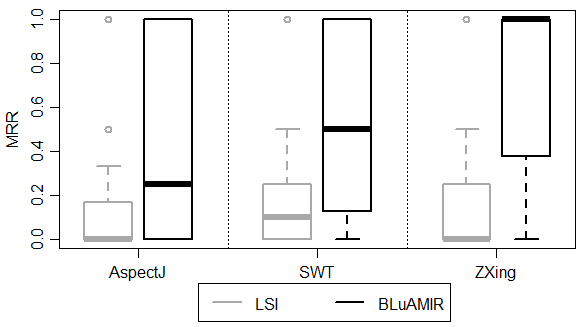
\includegraphics[width=3in]{comapre-mrr}
	\vspace{-.3cm}
	\caption {Comparison between baseline LSI and proposed approach, BLuAMIR, in MRR}
	\label{box:LSI+AssoMRR}
	\vspace{-.1cm}
\end{figure}
\begin{figure}
	\centering
	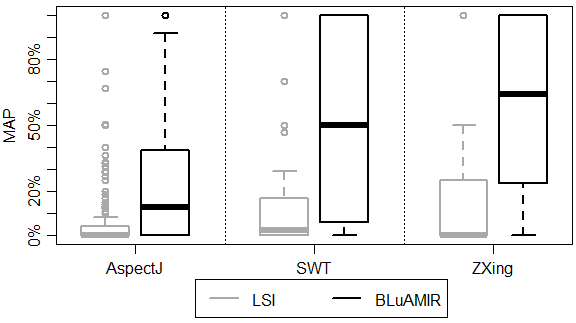
\includegraphics[width=3in]{compare-map-lsi-proposed}
	\vspace{-.3cm}
	\caption {Comparison between baseline LSI and proposed approach, BLuAMIR, in MAP}
	\label{box:LSI+Asso-MAP}
	%\vspace{-.5cm}
\end{figure}

\FrameSep3pt
\begin{framed}
	\noindent
	\textbf{Summary of RQ$_1$:} Our approach outperforms two baseline approaches \cite{vector-space-model,MarcusLSI} with statistically significant, large margins. BLuAMIR can even deliver \textbf{10\%--55\%} higher Hit@10, \textbf{15\%--163\%} higher MRR and \textbf{13\%--194\%} higher MAP than the baseline.  
\end{framed}
%\textbf{Wilcoxon signed-rank test}
%The Wilcoxon signed-rank test is a non-parametric statistical hypothesis test used to compare two related samples, matched samples, or repeated measurements on a single sample to assess whether their population mean ranks differ. We perform this test with the help of \footnote{https://www.socscistatistics.com/tests/signedranks/Default.aspx}.
%
%\textbf{Cross Validation}
%We divide our query data into k number of sets. Typically k is 10, but we work with k =5 and k=10. Each set contains a training set and tesing set. Training data is used to create mapping between keywords extracted from bug reports and source code files. 10-fold-cross validation data is presented in table \ref{tab:Performance1} and table \ref{tab:Performance2}.
\begin{table}[!tb]
	\centering
	\caption{Comparison with State-of-the-art}
	\vspace{-.2cm}
	\label{tab:performance3}
	\resizebox{3.35in}{!}{%
		\begin{tabular}{l|l|c|c|c|c|c}
			\hline
			%\begin{tabular}[c]{@{}c@{}}\#Bugs for \\ developing \\ map databases\end{tabular} &
			
			\begin{tabular}[c]{@{}c@{}}\textbf{System}   \\ \end{tabular} & 
			\begin{tabular}[c]{@{}c@{}}\textbf{Approach}\end{tabular} 
			& 
			\begin{tabular}[c]{@{}c@{}}\textbf{Hit@1}\end{tabular} & \begin{tabular}[c]{@{}c@{}}\textbf{Hit@5}\end{tabular} & \begin{tabular}[c]{@{}c@{}}\textbf{Hit@10}\end{tabular} & 
			\textbf{MRR} 
			& \textbf{MAP} \\ \hline \hline
			\multirow{4}{*}{Eclipse}                                       
			%& LSI &   &  &  &  &  \\  \cline{2-7} 
			& BugScout & 14.00 & 24.00 &  31.00 & -- & -- \\  \cline{2-7} 
			& BugLocator & 24.36 & 46.15 & 55.90 & 0.35 & 0.26 \\  \cline{2-7} 
			& BLUiR & 30.96  & 53.20 & 62.86  & 0.42 & 0.32 \\  \cline{2-7}
			&BLuAMIR                                                                     & 27.45                                               & \textbf{53.79}                                              & \textbf{63.30}                                            &   0.38  &   0.27  \\ \hline \hline
			\multirow{4}{*}{AspectJ}                                       
			%& LSI &  &  &  &  &  \\  \cline{2-7} 
			& BugScout & 11.00 & 26.00 & 35.00 & -- & -- \\  \cline{2-7}
			& BugLocator & 22.73 & 40.91 & 55.59 & 0.33 & 0.17 \\  \cline{2-7} 
			& BLUiR & 32.17 & 51.05 & 60.49 & 0.41 & 0.24 \\  \cline{2-7}
			&BLuAMIR                                                                     & \textbf{33.20}                                               & \textbf{54.92}                                              & \textbf{66.39}                                             &   \textbf{0.43}  &   0.23  \\ \hline \hline
			\multirow{4}{*}{SWT}                                       
			% & LSI & 13.26 & 30.61 & 53.06 & 0.15 & 0.14 \\  \cline{2-7} 
			
			& BugLocator & 31.63 & 65.31 & 77.55 & 0.47 & 0.40 \\  \cline{2-7} 
			& BLUiR & 55.10 & 76.53 & 87.76 & 0.65  & 0.56 \\  \cline{2-7} &BLuAMIR                                                                     & 45.93                                               & 75.00                                              & 82.29                                             &   0.58  &   0.50  \\ \hline \hline
			\multirow{4}{*}{ZXing}                  
			
			
			% & LSI & 15.00& 35.00 & 45.00 & 0.23 & 0.23 \\  \cline{2-7}  
			& BugLocator & 40.00 & 55.00 & 70.00 & 0.48 & 0.41 \\  \cline{2-7}  
			& BLUiR & 40.00 & 65.00 & 70.00 & 0.49  & 0.38 \\  \cline{2-7}
			&BLuAMIR                                                                  & \textbf{55.00}                                            & \textbf{80.00}                                           & \textbf{85.00}                                             &   \textbf{0.67}  &  \textbf{0.62}   \\ \hline
			
			
			
			
		\end{tabular}
		
	}
	%\vspace{-.5cm}
	\centering
\end{table}
%\subsection{Answering RQ4}\label{RQ4answer}
\textbf{Answering RQ$_2$-- Comparison with the State-of-the-Art:} While the above evaluation clearly shows that our approach is promising, we still wanted to see where our method stands compared to the state-of-the-art methods. Thus, 
we compare BLuAMIR with three state-of-the-art techniques -- BugScout \cite{Nguyen}, BugLocator \cite{Jian} and BLUiR \cite{Saha} -- using our benchmark subject systems. 
BugScout employs Latent Dirichlet Allocation (LDA) for localizing software bugs. BugLocator combines a revised Vector Space Model (rVSM) and past bug reports for improving the IR-based bug localization. Finally, BLUiR exploits the structures from both bug reports (queries) and source code documents, and then improves the bug localization with structured information retrieval.    
Table \ref{tab:performance3} summarizes our comparison details.
\citet{Nguyen} used two subject systems (Eclipse and AspectJ) in order to evaluate BugScout.
Both \citet{Saha} and \citet{Jian} employ all four subject systems for their evaluation. Since we use the same dataset from the earlier studies \cite{Saha,Jian}, we compare with their published results. 

\begin{table*}[!tb]
	\centering
	\caption{Comparison of Result Rank Improvement with State-of-the-art on Eclipse System}
	\vspace{-.4cm}
	\label{tab:Query-Rank}
	\resizebox{6in}{!}{%
		\begin{tabular}{l|c||c|c|c|c||c|c|c|c||c}
			\hline
			\multirow{2}{*}{\textbf{Approach}}
			& \multirow{2}{*}{\textbf{\#Bugs}}
			& \multicolumn{4}{c||}{\textbf{Improvement}}
			
			& \multicolumn{4}{c||}{\textbf{Worsening}}
			
			& \multirow{2}{*}{\textbf{\# Preserved}}  \\
			\hhline{~~--------~}
			& & \textbf{\#Improved} 
			& \textbf{Mean}
			& \textbf{Min.} 
			& \textbf{Max.}
			& \textbf{\#Worsened} 
			& \textbf{Mean}   
			& \textbf{Min.} 
			& \textbf{Max.} 
			& \\
			\hline \hline
			BugLocator & 
			2911 &
			1315 (45.17\%)	&
			68.46&
			1	&
			949	&
			1084 (37.23\%)	&
			172.87	&
			1	&
			8030	&
			512 (17.59\%)	\\ \hline
			%			BLUiR & 
			%			3,075 &
			%			&
			%			&
			%			&
			%			&
			%			&
			%			&
			%			&
			%			&
			%			\\ \hline
			BLuAMIR & 
			2864 &
			1328 (46.37\%) &
			50.90 &
			1 &
			909 &
			763 (26.64\%) &
			52.10 &
			1 &
			811 &
			773 (26.99\%)\\
			\hline
		\end{tabular}
	}
	\vspace{-.1cm}
	\centering
\end{table*}


From Table \ref{tab:performance3}, we see that BLuAMIR outperforms both BugScout and BugLocator consistently across all the systems (Eclipse, AspectJ, SWT and Zxing) and all performance metrics.
%dataset in three performance metrics (i.e., Hit@1, Hit@5 and Hit@10). 
BugLocator is a common baseline for a number of existing studies \cite{Saha,Wang2,Wang}. BugLocator performs the best with \emph{SWT} system, and achieves 78\% Hit@10 with a MRR of 0.47 and a MAP of 0.40. On the contrary, BLuAMIR achieves 82\% Hit@10 with a MRR of 0.58 and a MAP of 0.50 which are 6\%, 23\% and 25\% higher respectively. We also see that our approach performs better than BLUiR with three out of four systems--Eclipse, AspectJ and ZXing--in terms of several performance metrics (i.e., emboldened measures). While BLUiR performs better than ours with SWT system, it only contains 98 bug reports. On the contrary, AspectJ contains 2.5 times more bug reports, and our approach outperforms BLUiR with this system. For example, while BLUiR achieves 60\% Hit@10, our approach improves upon this metric by 10\% which is promising.      
%For AspectJ and SWT dataset, we can see our tool BLuAMIR outperforms BLUiR \cite{Saha} for Hit@1, Hit@5, Hit@10 and MRR@10. However, though BLuAMIR shows higher precision (i.e., MAP) than BLUiR \cite{Saha} for Zxing dataset, this also shows comparable precision with BLUiR \cite{Saha} for AspectJ.
%For Eclipse dataset BLuAMIR produce better results than BLUiR \cite{Saha} for Hit@5 and Hit@10 retrieval, but BLUiR \cite{Saha} shows better performance than BLuAMIR for Hit@1, MRR and MAP. On the other hand, for SWT dataset BLuAMIR shows comparable performance for Hit@5 and does not outperform for Hit@1, Hit@10, MRR and MAP. 
We also investigate why our approach fails to outperform BLUiR with SWT system. In particular, we calibrate the weighting parameter $\alpha$ and demonstrate that BLuAMIR could perform comparably with BLUiR with the right $\alpha$ value. Table \ref{tab:SWTalpha} summarizes our investigation results. We see that our approach delivers improved Hi@1, Hit@5, MAP and MRR at $alpha$ = $0.2$. However, it achieves the highest Hit@10 (85\%) at $alpha$ = $0.3$, which is comparable to that (88\%) of BLUiR \cite{Saha}. Thus, choosing the right $\alpha$ needs significant trade-off which we leave as an area for future study. However, such investigation clearly states that our approach has a high potential for bug localization. 

\begin{table}[!tb]
	\centering
	\caption{Impact of Weighting Parameter on BLuAMIR (with SWT System) }
	\vspace{-.2cm}
	\label{tab:SWTalpha}
	\resizebox{2.8in}{!}{%
		\begin{tabular}{c|l|c|c|c|c}
			\hline
			%\begin{tabular}[c]{@{}c@{}}\#Bugs for \\ developing \\ map databases\end{tabular} &
			{$\alpha$} 
			
			& \textbf{Hit@1} 
			& \textbf{Hit@5}  & 
			\textbf{Hit@10}  &
			\textbf{MRR}  & 
			\textbf{MAP}  \\
			\hline
			\hline
			{0.1} 
			& 43.75                                            & 73.96                                            & 83.33                                                &   0.57  & 0.50    \\ \hline
			{0.2} 
			& 48.96                                               & 75.00                                              & 83.33                                             &   0.60  &   0.51  \\ 
			\hline
			{0.3} 
			
			&47.92 &
			72.92 &
			85.42 & 0.59 &
			0.51     \\  
			\hline
			{0.4}      
			& 45.93                                                 & 75.00                                                 & 82.29                                                  &   0.58  &  0.50    \\ 
			\hline
	\end{tabular}}
	\vspace{-.1cm}
	\centering
\end{table}

We also investigate how each of the three approaches -- BugLocator, BLUiR and BLuAMIR -- improve upon baseline VSM in terms of result rank improvement for the queries of Eclipse system. In particular, we (1) collect the rank of first correct buggy document within the results returned by baseline VSM (i.e., baseline rank), and (2) collect similar rank for each of these approaches (i.e., changed rank), and (3) then determine the result improvement and worsening by comparing the changed ranks with the baseline ranks. Table \ref{tab:Query-Rank} contrasts our approach with the state-of-the-art in terms of result rank improvement and worsening. We see that BugLocator improves upon VSM for 45.17\% of the queries and worsens 37.23\% of the queries. On the contrary, BLuAMIR improves 46.37\% and worsens 26.64\% of the queries which are 2.66\% higher and 39.75\% lower respectively. All these findings clearly suggest the high potential of our approach in bug localization.    

\FrameSep3pt
\begin{framed}
	\noindent
	\textbf{Summary of RQ$_2$:} Our approach outperforms two of the state-of-the-art studies \cite{Nguyen,Jian} and performs comparably with one study \cite{Saha}. BLuAMIR not only achieves \textbf{23}\% higher MRR but also delivers \textbf{25}\% higher MAP than the state-of-the-art. 
	%improves the results of \textbf{2.66}\% more queries.
	%two baseline approaches with statistically significant, large margins. BLuAMIR can even deliver \textbf{10\%--55\%} higher Hit@10, \textbf{15\%--163\%} higher MRR and \textbf{13\%--194\%} higher MAP than the baseline approaches.  
\end{framed}

\textbf{Answering RQ3-(a) Impact of Association Score on Bug Localization:} 
<<<<<<< HEAD
While the above two findings suggest that our proposed approach is highly potential in bug localization, at this point we wanted to investigate why our proposed approach outperforms than the lexical similarity-based state-of-the-art methods. 
Note that in our proposed approach, we make use of not only the lexical similarity but also the implicit association between a bug report and the source code from the bug fixing history. We still wanted to see, is implicit association making any significant difference in IR-based bug localization? 
This implicit association capture the historical relevance between the query keywords and their corresponding source code, based on bug-fixing history. It should be noted that such relevance does not warrant for lexical similarity. 
We investigate the impact of association score on the bug localization performance of our approach across multiple subject systems. 
In particular, we tune our approach with different $\alpha$ values, and record the responses. Since $\alpha$ is the relative weight of association score, such tuning actually evaluates the impact of association score.  
=======
While RQ$_1$ and RQ$_2$ suggest that our proposed approach has high potential for bug localization, at this point, we wanted to investigate in-depth why our proposed approach performs better than the lexical similarity-based approaches. We make use of 
not only the lexical similarity but also the implicit association between a bug report (query) and the source code that is derived from the bug fixing history. Thus, in this RQ, we wanted to see whether such implicit association has any significant impact on the bug localization performance or not. 
%making any significant difference in IR-based bug localization? 
%This implicit association capture the historical relevance between the query keywords and their corresponding source code, based on bug-fixing history. It should be noted that such relevance does not warrant for lexical similarity. 
%Thus, we investigate the impact of association score on the bug localization performance of our approach across multiple subject systems. 
In particular, we tune our approach with different $\alpha$ values, and record the responses. Since $\alpha$ is the \emph{relative weight} of \emph{association score}, such tuning actually evaluates the impact of association score.  
>>>>>>> 81be3cfef1546cb078b22a794d11382f0ccc3ea7
Table \ref{tab:alphaApproach1} shows how the gradual increment in $\alpha$ value improves the overall performance. We see that each of the metrics improves consistently up to $\alpha$ = 0.4 with Eclipse system. 
\begin{table}[!tb]
	\centering
	\caption{Impact of Weighting Parameter on BLuAMIR (with Eclipse System)}
	\vspace{-.2cm}
	\label{tab:alphaApproach1}
	\resizebox{2.8in}{!}{%
		\begin{tabular}{c|l|c|c|c|c}
			\hline
			%\begin{tabular}[c]{@{}c@{}}\#Bugs for \\ developing \\ map databases\end{tabular} &
			{$\alpha$} 
			
			& \textbf{Hit@1}  
			& \textbf{Hit@5} & 
			\textbf{Hit@10}  &
			\textbf{MRR}  & 
			\textbf{MAP}  \\
			\hline
			\hline
			{0.0} &21.20& 43.05& 54.58&0.31&0.22 \\ \hline
			{0.1} &22.83& 46.47 & 58.02& 0.33& 0.23 \\ \hline
			{0.2} 
			& 24.23                                            & 49.53                                            & 60.44                                                &   0.35  & 0.25    \\ \hline
			{0.3} 
			& 25.72                                               & 51.87                                              & 62.45                                             &   0.37  &   0.27  \\ 
			\hline
			{0.4} 
			
			
			&27.45 &
			53.79 &
			63.30 & 0.38 &
			0.27     \\  
			\hline
			%{Average}      & 25.80\%                                                 & 51.73\%                                                 & 62.06\%                                                  &   0.37  &  0.26    \\ 
			%\hline
	\end{tabular}}
	\centering
\end{table}
\begin{figure}[!t]
	\centering
	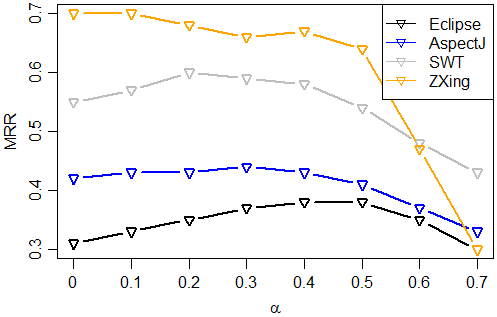
\includegraphics[width=2.5in]{alpha-calibration-mrr}
	\vspace{-.3cm}
	\caption{The impact of $\alpha$ on BLuAMIR's MRR}
	\label{fig:MRR-alpha-cali}
	\vspace{-.3cm}
\end{figure}
\begin{figure}[!t]
	\centering
	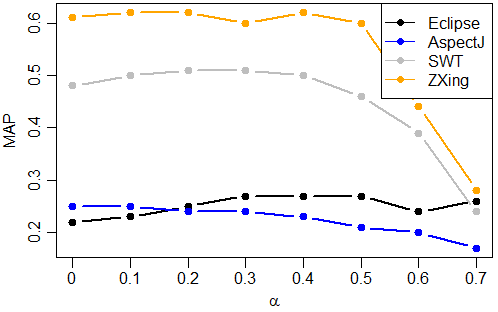
\includegraphics[width=2.5in]{alpha-calibration-map}
	\vspace{-.3cm}
	\caption{The impact of $\alpha$ on BLuAMIR's MAP}
	\label{fig:MAP-alpha-cali}
	%\vspace{-.5cm}
\end{figure}
We also repeat the same investigation with different $\alpha$ values with all four systems. From Fig. \ref{fig:MRR-alpha-cali}, we see that BLuAMIR initially performs low with $\alpha$ = 0, i.e., no association score. Then our MRR improves continuously with the increment of $\alpha$. We see a somewhat stationary state during 0.2$\le\alpha\le$0.4 followed by a sharp decrease in MRR with all systems except Eclipse.
This performance reaches the lowest at $\alpha$ = 0.7.
We also note a pretty similar scenario in Fig. \ref{fig:MAP-alpha-cali} when investigated with MAP.
Such findings above suggest that association score has a noticeable impact upon the bug location performance. That is, lexical similarity + association score is consistently better than lexical similarity alone. Our findings in RQ$_1$ also support this observation with empirical evidence. Such findings also justify our choice for $\alpha$ between 0.2 and 0.4 in our approach. 

\textbf{(b) Overcoming the Challenge with Large Documents:}
We further wanted to investigate whether our approach could work well with large source documents. This is in particular important to investigate since traditional VSM approaches are mostly biased towards such large source documents during bug localization. 
%Traditional VSM approaches are generally biased towards large source documents during bug localization. 
Although these documents have a major overlap with a given bug report (query), they are often noisy and less relevant in practice. We discuss how BLuAMIR can overcome this challenge during bug localization with an example as follows:

\textbf{A Case Study with Large Documents:} Let us consider a bug report (ID \#95561) from \texttt{eclipse.ui.platform} subsystem of Eclipse. The bug report discusses about a synchronization issue with Eclipse workbench. We preprocess the \emph{title} and \emph{description} of the bug report, and use them as the query for bug localization. According to the bug-fixing history, \texttt{org.eclipse.ui.internal.WorkbenchPage.java} constitutes the ground truth for this query, which is a large document with 4K+ lines of code and $\approx$14K words. Baseline VSM \cite{vector-space-model} and BugLocator \cite{Jian} return this ground truth at the 30$^{th}$ and 26$^{th}$ positions respectively. On the contrary, our approach returns the same ground truth at the second position of the result list which is promising. We then perform in-depth analysis on the ranking mechanism of each approach, and make interesting observations. First, the lexical score for this document is 0.45 due to noise, which is much lower than that of the other smaller candidate documents. Such a low score possibly pushes the document down the ranked list. On the contrary, BLuAMIR complements such low lexical scores with a strong association score of 0.95. The document and the query are strongly associated according to the bug-fixing history. Thus, final score for the document is calculated by BLuAMIR as follows:  (0.95$\times$0.40+0.45$\times$0.60) = 0.65. Such a final score places the candidate source document at the second position in our case. Thus, \emph{implicit association} dimension can actually help overcome the challenges (noises) with large source documents. 

\FrameSep3pt
\begin{framed}
	\noindent
	\textbf{Summary of RQ$_3$:} Our empirical and analytical findings suggest that \textbf{implicit association} can make a significant difference to IR-based bug localization by (a) \textbf{improving} upon baseline VSM and (b) \textbf{overcoming} the challenges with large candidate documents.    
\end{framed}

\section{Threats To Validity}\label{sec:threats}
This section discusses the validity and generalizability of our findings. In particular, we discuss the threats to internal validity, construct validity, and external validity as follows:

\textbf{Internal Validity:} We used three artifacts of a software repository: bug reports, source code documents and bug fixing history, which are generally well understood. Our evaluation uses four open source subject systems - Eclipse, AspectJ, SWT, and ZXing. These systems are collected from two existing, frequently used public benchmarks \cite{Jian, Saha}. 
Bug reports provide crucial information for developers to fix the bugs.
A bug report could be of low quality and could miss the appropriate keywords.
Hence, such a “bad” bug report could cause a delay in the bug fixing process. Our proposed approach makes use of both lexical similarity as well as implicit association between a bug report and their corresponding source code documents. Therefore, if a bug report does not provide adequate information, or provides inappropriate keywords, the performance of BLuAMIR could be adversely affected.

\textbf{External Validity:} 
Threats to external validity is related to the generalizability of our findings. 
To reduce this threat, we have analyzed 3,431 bug reports from four popular subject systems.  
Still in the future, we plan to reduce these threats further by analyzing more bug reports from more subject systems written in multiple programming languages.

%The nature of the data in open source projects may be different from those in projects developed by well-managed software organizations. We need to evaluate if our solution can be directly applied to commercial projects. We leave this area as a future study. 
%Then we will perform statistical tests to show that the improvement of our approach is statistically significant.

\textbf{Construct Validity:}
In our experiment, we use three evaluation metrics -- Hit@K, MAP and MRR, and one statistical test, i.e., Wilcoxon signed-rank test. These metrics have been widely used in the literature to evaluate bug localization performances \cite{Jian, Saha}. Thus, threats to construct validity are likely to be mitigated.

%we argue that our research has strong construct validity.

\textbf{Parameter Tuning:}
We tune our weighting parameter using controlled iterative experiments, and report our findings (Section \ref{RQ1answer}).
However, such iterative experiments might not guarantee an optimal parameter value. In future, we plan to use more sophisticated parameter tuning methods such as Genetic Algorithms. 


%In our experiment, we performed numerous experiments using various combinations of weighting functions to find the optimum parameters and the best accuracy of bug localization. 
%The optimized $\alpha$ values are based on our experiments and are only for our proposed tool BLuAMIR. 
%To automatically optimize control parameters for target projects, in the future we will expand our proposed approach using machine learning methods or generic algorithms.

\section{Related Work}\label{relatedwork}
Existing automatic bug localization or automatic debugging approaches can be broadly categorized into two types - dynamic and static techniques. Generally, dynamic approaches can localize a bug much more precisely than static approaches. These techniques usually contrast the program spectra information (such as execution statistics) between passed and failed executions to compute the fault suspiciousness of individual program elements (i.e., statements, branches, and predicates), and rank these program elements by their fault suspiciousness. Developers may then locate faults by examining a list of program elements sorted by their suspiciousness. Some of the well known dynamic approaches are spectrum-based fault localization \cite{Abreu,Jones,Lucia,SahaFault}, model-based fault localization \cite{Feldman,Mayer}, dynamic slicing \cite{Zhang:2005}, and delta debugging \cite{Zeller:2002}. These approaches require a test case suite and need to execute the program for collecting the passed and failed execution traces. Moreover, these approaches are computationally expensive. 
%Neither our proposed approach requires a test case nor computationally expensive.
Our proposed approach neither requires a test case nor requires the execution of the program. 


Static approaches, on the other hand, do not require any program test cases or execution traces. In most cases, they need only program source code documents and bug reports. They are also computationally efficient. The static approaches usually can be categorized into two groups: program analysis based approaches and IR-based approaches. FindBugs is a program analysis based approach that locates a bug based on some predefined bug patterns \cite{FindBug}. 
Therefore, FindBug does not even need a bug report. However, it often detects too many false positives and misses many real bugs \cite{Tang}. 
%On the contrary, our proposed technique does not depend on any predefined bug patterns. Thus, our proposed approach does not produce too many false positive results 
%and particularly, it does not miss too many bugs. 
%and, in particular, it does not miss too many bugs.
On the contrary, our proposed approach is not program analysis based, and thus, does not depend on any predefined bug patterns.

Traditional Information Retrieval based techniques localize the bugs by simply relying on the \emph{lexical similarity} between a bug report (query) and the source code. 
There are three traditionally-dominant IR paradigms: TFIDF \cite{Salton}, the probabilistic approach known as BM25 \cite{Robertson}, and more recently, language modeling \cite{Ponte}. However, using an empirical study, \citet{Fang} show that all three approaches perform comparably when well-tuned. On the other hand, \citet{Rao} investigated many standard information retrieval techniques for bug localization and found that simpler techniques, e.g., TFIDF and SUM, perform the best. However, If a bug report does not contain adequate information (i.e., appropriate keywords), lexical similarity alone might not be sufficient enough to localize the bugs successfully. In order to address the issue with lexical similarity, 
%In contrast with shallow “bag-of-words” models, 
Latent Semantic Indexing (LSI) introduces latent concepts by exploring deeper methods matching ``concepts". While a probabilistic variant of LSI has been devised \cite{Hofmann}, its probability model was found to be deficient. On the other hand, several other studies \cite{Maletic, MarcusMaletic,irmarcus} derive the underlining semantic of a text document by employing Latent Semantic Analysis (LSA).
Unfortunately, their approach suffers from a major limitation.
Latent Semantic Indexing (LSI) requires the use of a dimensionality reduction parameter that must be tuned for each document collection \cite{Kontostathis}.
The results returned by LSI can also be difficult to interpret, as
they are expressed using a numeric spatial representation.
Our approach does not require dimensionality reduction since we use a finite graph rather than a large sparse term-document matrix \cite{MarcusLSI,MarcusMaletic}.
%On the other hand, \citet{Lukins} created a Latent Dirichlet Allocation (LDA) model from the source code which provided word-topic modeling and topic-document distribution.
%\citet{Lukins2} use Latent Dirichlet Allocation (LDA), which is a well-known topic modeling approach, to localize bug. 
\citet{LukinsBL} and \cite{Nguyen} adopt Latent Dirichlet Allocation (LDA) for bug localization. LDA is not able to predict the appropriate topic because it follows a generative topic model in a probabilistic way \cite{Lukins}. Besides, they are also subject to their hyper-parameters and could even be outperformed by simpler models (e.g., rVSM \cite{Jian}).  
LDA is also computationally expensive. In this paper, we compare with a baseline LSI \cite{MarcusLSI} and a LDA based technique namely BugScout \cite{Nguyen} and the detailed comparison can be found in Section \ref{RQ1answer} (i.e., RQ1 and RQ2 respectively). Our approach outperforms both these baseline\cite{MarcusLSI,Nguyen} with large margins across all subject systems. 

Recently automatic bug localization techniques have gone beyond traditional
Information Retrieval based techniques by collecting additional information from software repositories \cite{Sisman, Jian, Saha, Moreno, Wang}.
\citet{Sisman} propose a history-aware IR-based bug localization solution to achieve a better
result. \citet{Jian} propose BugLocator, which leverages similarities among bug reports and uses a refined vector space model to perform bug localization. \citet{Saha} build BLUiR that considers the structure of bug reports and source code files and employs structured retrieval to achieve a better result. \citet{Moreno} use a text retrieval based technique and stack trace analysis to perform bug localization. To locate buggy files, they combine the textual similarity between a bug report and a program entity (e.g., class) and the structural similarity between the stack trace and the entity. Different from the existing IR-based bug localization approaches, \citet{Wang} proposed AmaLgam, a new method for locating relevant buggy files that puts together version history, similar reports, and structure, to achieve better performance. 
%Later \cite{Wang2} also propose AmaLgam+
Later, they proposed AmaLgam+\cite{Wang2}, which is a method for locating relevant buggy files that puts together fives sources of information i.e., version history, similar reports, structure, stack traces, and reporter information. 
However, in our proposed technique BLuAMIR, we consider only three sources of information i.e., bug reports, source code documents and bug fixing history. 
Hence, we performed extensive comparison with two closely related studies -- BugLocator \cite{Jian} and BLUiR\cite{Saha}.
The details of our comparison can be found in Section \ref{RQ1answer} (i.e., RQ2).
Unlike the above traditional IR-based approaches \cite{Sisman, Jian, Saha, Moreno, Wang, Wang2}, our proposed approach could deliver the buggy documents even if the bug report (the query) does not lexically match with source code documents.
Our proposed approach outperforms BugLocator \cite{Jian} consistently across all the subject systems. BLuAMIR also performs better than BLuIR \cite{Saha} with three out of four subject systems and perform comparably with the remaining system.

\section{Conclusion and Future Work} \label{sec:conclusionANDfuture}
During the evolution of a software system, a large number of bug reports are submitted. For a large software project, developers typically need to examine a large number of source code files in order to locate the buggy files responsible for a bug, which is tedious and expensive work. In this paper, we propose BLuAMIR, a new bug localization technique not only based on lexical similarity but also on an implicit association mapping between bug report keywords and source code documents. We perform large-scale experiments with four subject systems, namely Eclipse, SWT, AspectJ and ZXing to localize 3,431 bug reports.
We also compare our technique with two baseline techniques i.e., \cite{vector-space-model}, \cite{MarcusLSI}, and three state-of-the-art IR-based bug localization techniques i.e., BugScout\cite{Nguyen}, BugLocator\cite{Jian} and BLUiR\cite{Saha}.
Our experiment with those dataset shows that on average our technique can locate buggy files with a Top-10 accuracy of 74.06\% and a mean reciprocal rank of 0.52 and a mean precision average of 41\%, which is highly promising.   
%This also confirms superiority of our technique. 
Our technique can localize bugs with 6\%--54\% higher accuracy (i.e., Hit@5), 4\%--32\% higher precision (i.e., MAP) and 8\%--27\% higher reciprocal ranks (i.e., MRR) than these state-of-the-art approaches. All these empirical findings suggest the high potential of our proposed approach for bug localization. 

In the future, we will explore whether other bug related information such as bug report structure, source code structure, stack traces, reporter information, and similar bug information could be integrated into our approach or not. Such external resources could also assist in handling the vocabulary mismatch issues and the challenges with poor queries.

\balance


%
% The next two lines define the bibliography style to be used, and the bibliography file.
\bibliographystyle{ACM-Reference-Format}
\bibliography{test}





\end{document}
